\chapter{CƠ SỞ LÝ THUYẾT}

\section{Tổng quan về gom cụm dữ liệu}
\subsection{Khái niệm và mục tiêu của gom cụm dữ liệu}

Gom cụm (Clustering) là cách chia các điểm dữ liệu thành những nhóm dựa trên đặc điểm của chúng. Đây là học không giám sát vì ban đầu không có nhãn cho biết mỗi điểm thuộc nhóm nào; thuật toán tự tìm các nhóm từ dữ liệu.

Xét tập dữ liệu \(D\) gồm \(n\) đối tượng, trong đó mỗi đối tượng \(x_i\) được mô tả bằng \(d\) giá trị số thực:

\begin{equation}
    D = \{x_1, x_2, \ldots, x_n\}, \qquad x_i \in \mathbb{R}^{d}.
\end{equation}

Trong phạm vi đồ án, nhóm sử dụng cách gom cụm mà trong đó mỗi đối tượng được gán vào tối đa một cụm. Đối với các thuật toán cho phép nhận diện nhiễu, kết quả gom cụm có thể được biểu diễn như sau:

\begin{equation}
    D = \left(\bigcup_{j=1}^{k} C_j\right) \cup {N},
    \qquad
    C_i \cap C_j = \varnothing \quad (i \neq j),
    \qquad
    C_j \cap {N} = \varnothing.
\end{equation}

Trong đó, \(C_j\) là cụm thứ \(j\), \(k\) là số cụm được hình thành và \(N\) là tập các đối tượng không thuộc cụm nào, được gọi là nhiễu (Noise). Các điều kiện trên cho biết mỗi đối tượng chỉ thuộc tối đa một cụm, đồng thời không thể vừa thuộc một cụm vừa được xác định là nhiễu.

DBSCAN cho phép đánh dấu những điểm không thuộc cụm nào là nhiễu. Nếu mọi điểm đều được đưa vào cụm thì tập nhiễu có thể rỗng.

Việc xác định các đối tượng thuộc cùng một cụm phụ thuộc vào cách thuật toán định nghĩa sự tương đồng. Ví dụ, K-means sử dụng khoảng cách đến tâm cụm, trong khi các thuật toán gom cụm phân cấp có thể dựa trên khoảng cách hoặc quan hệ liên kết giữa các nhóm đối tượng. Đối với DBSCAN, các cụm được hình thành dựa trên mật độ và quan hệ khả đạt theo mật độ giữa các đối tượng.

Sự khác biệt này có ý nghĩa trong việc đánh giá cấu trúc cụm. Hai đối tượng nằm ở hai đầu một cụm có thể cách nhau khá xa nhưng vẫn có thể thuộc cùng một cụm nếu tồn tại chuỗi kết nối theo mật độ giữa chúng. Vì vậy, tính tương đồng trong gom cụm không nhất thiết đòi hỏi mọi cặp đối tượng trong cùng một cụm phải có khoảng cách nhỏ. Tiêu chí hình thành cụm cần được xem xét theo nguyên lý của từng thuật toán.

Trong đồ án này, nhóm tập trung vào phương pháp phân cụm dựa trên mật độ, đặc biệt là DBSCAN và phiên bản cập nhật tăng dần Incremental DBSCAN.

\subsection{Các phương pháp gom cụm phổ biến}

Các thuật toán gom cụm có thể được phân biệt dựa trên cách xác định sự tương đồng và tổ chức các đối tượng thành cụm. Trong đó, ba loại phổ biến là gom cụm theo phân hoạch, gom cụm phân cấp và gom cụm dựa trên mật độ. Mỗi loại sử dụng một nguyên tắc hình thành cụm khác nhau, do đó có thể tạo ra những kết quả khác nhau khi áp dụng trên cùng một tập dữ liệu.

\textbf{Gom cụm theo phân hoạch (Partitioning Clustering)}

Phương pháp gom cụm theo phân hoạch chia tập dữ liệu thành một số cụm xác định. Ví dụ là K-means, trong đó mỗi đối tượng được cho vào cụm có tâm gần nhất và các tâm cụm được cập nhật qua nhiều lần lặp. Phương pháp này yêu cầu xác định trước số lượng cụm \(k\) và thường phù hợp với các nhóm dữ liệu phân bố tập trung quanh một tâm, nhưng có thể gặp hạn chế khi các cụm có hình dạng phức tạp.

\textbf{Gom cụm phân cấp (Hierarchical Clustering)}

Phương pháp gom cụm phân cấp xây dựng cấu trúc thể hiện quan hệ giữa các cụm nhỏ và những cụm lớn được hình thành từ chúng. Ví dụ như trong thuật toán gom cụm phân cấp kết tụ (Hierarchical Agglomerative Clustering – HAC), ban đầu mỗi đối tượng được xem là một cụm riêng, sau đó các cụm được hợp nhất dần dựa trên tiêu chí liên kết đã chọn. Quá trình này được biểu diễn bằng cấu trúc cây cho phép quan sát thứ tự và mức khoảng cách mà các cụm được hợp nhất.

\textbf{Gom cụm dựa trên mật độ (Density-Based Clustering)}

Thay vì xác định cụm thông qua tâm đại diện hoặc trình tự hợp nhất các nhóm, phương pháp dựa trên mật độ xét sự phân bố của các đối tượng trong những vùng lân cận. Các vùng có đủ mật độ và có quan hệ kết nối với nhau được xác định thuộc cùng một cụm, trong khi những đối tượng không đáp ứng điều kiện tham gia cụm có thể được nhận diện là nhiễu.

DBSCAN thuộc nhóm thuật toán dựa trên mật độ. Thuật toán dùng các điểm lõi để mở rộng cụm, nên có thể tìm được cụm không tròn và không cần biết trước số cụm. Kết quả phụ thuộc vào bán kính lân cận và ngưỡng mật độ.

\section{Thuật toán DBSCAN}

DBSCAN (Density-Based Spatial Clustering of Applications with Noise) là thuật toán gom cụm dựa trên mật độ do Ester và cộng sự đề xuất. Thuật toán đếm các điểm ở gần nhau để tìm vùng đủ mật độ, mở rộng cụm từ các điểm lõi và đánh dấu các điểm không thuộc cụm là nhiễu \parencite{ester1996dbscan}.

Để thực hiện quá trình gom cụm, DBSCAN sử dụng hai tham số chính là \(\varepsilon\) (Eps) và \(\mathrm{MinPts}\). Hai tham số này quyết định điều kiện để một đối tượng có thể làm điểm bắt đầu mở rộng cụm, cũng như phạm vi các đối tượng được liên kết với nhau.

\subsection{Các tham số Eps và MinPts}

\textbf{Bán kính lân cận \(\varepsilon\) (Eps)}

\(\varepsilon\) (Eps) là ngưỡng khoảng cách dùng để xác định những đối tượng nằm trong lân cận của một đối tượng đang xét. Với tập dữ liệu \(D\) và hàm khoảng cách \(d\), lân cận \(\varepsilon\) của đối tượng \(p\), ký hiệu là \(N_{\varepsilon}(p)\), được định nghĩa:

\begin{equation}
    N_{\varepsilon}(p)
    = \{q \in D \mid d(p,q) \leq \varepsilon\}.
\end{equation}

Theo định nghĩa này, một đối tượng \(q\) sẽ thuộc \(N_{\varepsilon}(p)\) nếu khoảng cách từ \(p\) đến \(q\) không vượt quá \(\varepsilon\). Những đối tượng có khoảng cách lớn hơn \(\varepsilon\) sẽ không được xem là lân cận trực tiếp của \(p\).

Trong phạm vi cài đặt của nhóm, khoảng cách giữa hai đối tượng được tính bằng khoảng cách Euclid. Giả sử hai đối tượng \(p\) và \(q\) đều được mô tả bằng \(d\) giá trị số, khoảng cách giữa chúng được xác định như sau:

\begin{equation}
    d(p,q)
    = \sqrt{\sum_{j=1}^{d}(p_j-q_j)^2}.
\end{equation}

Trong đó, \(p_j\) và \(q_j\) lần lượt là giá trị thuộc tính thứ \(j\) của hai đối tượng, còn \(d\) là số chiều của dữ liệu. Công thức tính khoảng cách Euclid dựa trên độ chênh lệch giữa các thuộc tính tương ứng. Vì vậy, khi các thuộc tính có đơn vị hoặc thang đo khác nhau, những thuộc tính có giá trị số lớn có thể chi phối khoảng cách, từ đó ảnh hưởng đến kết quả xác định lân cận.

Ví dụ, trong không gian hai chiều, xét hai đối tượng \(p=(1;2)\) và \(q=(4;6)\):

\begin{equation}
    d(p,q)=\sqrt{(1-4)^2+(2-6)^2}=5.
\end{equation}

Nếu \(\varepsilon=5\) thì \(q\in N_{\varepsilon}(p)\). Ngược lại, nếu \(\varepsilon=4\) thì \(q\) không thuộc lân cận \(\varepsilon\) của \(p\). Như vậy, việc thay đổi \(\varepsilon\) có thể làm thay đổi số lượng đối tượng lân cận ngay cả khi dữ liệu không thay đổi.

Vì khoảng cách từ một điểm đến chính nó bằng 0, điểm đó cũng được tính trong lân cận của mình. Chương trình và các ví dụ của nhóm đều dùng quy ước này.

\textbf{Ngưỡng mật độ \(\mathrm{MinPts}\)}

\(\mathrm{MinPts}\) là số lượng đối tượng tối thiểu phải có trong lân cận \(\varepsilon\) để đối tượng đang xét được xác định là đối tượng lõi (Core).

Điều kiện xác định đối tượng lõi được biểu diễn như sau:

\begin{equation}
    |N_{\varepsilon}(p)| \geq \mathrm{MinPts}.
\end{equation}

Trong đó, \(|N_{\varepsilon}(p)|\) là số phần tử thuộc lân cận \(\varepsilon\) của \(p\), bao gồm cả chính \(p\). Điều kiện trên cho biết một đối tượng được xem là lõi khi số lượng đối tượng trong lân cận của nó đạt ít nhất ngưỡng \(\mathrm{MinPts}\).

\(\mathrm{MinPts}\) là ngưỡng để xác định một đối tượng có đủ điều kiện mật độ để trở thành lõi và mở rộng cụm hay không, chứ không phải là số lượng thành viên cố định của mỗi cụm. Một cụm hợp lệ phải chứa ít nhất MinPts đối tượng, nhưng có thể tiếp tục mở rộng qua nhiều đối tượng lõi liên tiếp và có số lượng thành viên lớn hơn ngưỡng này.

\textbf{Ảnh hưởng của hai tham số}

\(\varepsilon\) (Eps) và \(\mathrm{MinPts}\) quyết định mức mật độ tối thiểu mà DBSCAN sử dụng để nhận diện cụm. Nếu giữ nguyên \(\mathrm{MinPts}\) và giảm \(\varepsilon\), số đối tượng trong mỗi vùng lân cận thường giảm, khiến nhiều đối tượng không còn đủ điều kiện lõi. Ngược lại, tăng \(\varepsilon\) có thể làm xuất hiện thêm các kết nối giữa những đối tượng trước đó nằm ngoài lân cận của nhau.

Tương tự, khi giữ nguyên \(\varepsilon\), việc tăng \(\mathrm{MinPts}\) làm điều kiện trở thành lõi chặt chẽ hơn, còn giảm \(\mathrm{MinPts}\) khiến các đối tượng dễ thỏa mãn điều kiện lõi hơn. Vì vậy, hai tham số cần được xem xét cùng lúc vì thay đổi về mật độ có thể làm thay đổi cả số lượng cụm, thành viên cụm và số đối tượng được xác định là nhiễu.

\subsection{Đối tượng lõi, đối tượng biên và nhiễu}

Dựa trên số lượng đối tượng trong lân cận \(\varepsilon\) và quan hệ với những đối tượng lõi, DBSCAN phân biệt ba loại đối tượng: lõi (Core), biên (Border) và nhiễu (Noise).

\textbf{Đối tượng lõi (Core)}

Đối tượng \(p\) được xác định là lõi nếu:

\begin{equation}
    |N_{\varepsilon}(p)| \geq \mathrm{MinPts}.
\end{equation}

Đối tượng lõi có vai trò mở rộng cụm. Khi xét một đối tượng lõi, thuật toán có thể bổ sung các đối tượng nằm trong lân cận \(\varepsilon\) của nó vào cụm đang hình thành. Nếu trong số đó có đối tượng lõi khác, thuật toán tiếp tục xét lân cận của đối tượng lõi mới để mở rộng cụm.

\textbf{Đối tượng biên (Border)}

Đối tượng \(p\) được xác định là biên khi nó không thỏa mãn điều kiện lõi, nhưng nằm trong lân cận \(\varepsilon\) của ít nhất một đối tượng lõi \(q\):

\begin{equation}
\begin{aligned}
    |N_{\varepsilon}(p)| &< \mathrm{MinPts},\\
    \exists q \in D:\quad
    |N_{\varepsilon}(q)| &\geq \mathrm{MinPts}
    \quad \land \quad
    p \in N_{\varepsilon}(q).
\end{aligned}
\end{equation}

Điều kiện thứ nhất cho biết đối tượng \(p\) không có đủ số lượng đối tượng trong lân cận để trở thành lõi. Điều kiện thứ hai yêu cầu tồn tại ít nhất một đối tượng \(q\) trong tập dữ liệu \(D\), sao cho \(q\) có số lượng đối tượng trong lân cận lớn hơn hoặc bằng MinPts, tức là \(q\) là đối tượng lõi, đồng thời \(p\) nằm trong lân cận \(\varepsilon\) của \(q\). Khi thỏa mãn cả hai điều kiện, \(p\) được xác định là đối tượng biên.

Vì không đáp ứng điều kiện lõi, đối tượng biên được bổ sung vào cụm nhưng không được sử dụng để tiếp tục mở rộng cụm sang những đối tượng khác.

Trong một số trường hợp, một đối tượng biên có thể nằm trong lân cận của các đối tượng lõi thuộc những cụm khác nhau. Khi đó, đối tượng biên vẫn chỉ được gán vào một cụm, nhưng cụm được chọn có thể phụ thuộc vào thứ tự duyệt hoặc quy tắc gán nhãn của thuật toán.

\textbf{Nhiễu (Noise)}

Đối tượng được xác định là nhiễu nếu không phải lõi và cũng không nằm trong lân cận \(\varepsilon\) của bất kỳ đối tượng lõi nào. Khi đó, đối tượng không thuộc cụm nào theo các tham số đang sử dụng.

Trạng thái nhiễu trong kết quả cuối cùng khác với việc một đối tượng được đánh dấu nhiễu trong quá trình duyệt. Nếu thuật toán xét một đối tượng chưa đủ điều kiện lõi trước khi phát hiện cụm chứa nó, đối tượng đó có thể tạm thời được đánh dấu nhiễu. Sau đó, nếu một đối tượng lõi khác có lân cận chứa đối tượng này, nó vẫn được bổ sung vào cụm dưới dạng đối tượng biên.

Như vậy, việc một đối tượng không thỏa mãn điều kiện lõi chưa đủ để kết luận đối tượng đó là nhiễu. Thuật toán còn phải xét khả năng đối tượng được kết nối với một lõi khác.

\subsection{Nguyên lý mở rộng cụm}

Để hình thành một cụm hoàn chỉnh, DBSCAN cần xác định quan hệ giữa những đối tượng thông qua ba khái niệm: khả đạt trực tiếp theo mật độ, khả đạt theo mật độ và kết nối theo mật độ.

\textbf{Khả đạt trực tiếp theo mật độ (Directly Density-Reachable)}

Nói đơn giản, \(q\) khả đạt trực tiếp từ \(p\) khi \(p\) là lõi và \(q\) nằm trong bán kính \(\varepsilon\) của \(p\):

\begin{equation}
\begin{cases}
    q \in N_{\varepsilon}(p),\\
    |N_{\varepsilon}(p)| \geq \mathrm{MinPts}.
\end{cases}
\end{equation}

Quan hệ này có thể chỉ đi theo một chiều. Nếu \(p\) là lõi còn \(q\) là biên, \(q\) có thể được mở rộng từ \(p\), nhưng không thể dùng \(q\) để mở rộng ngược lại. Nếu cả hai đều là lõi và ở gần nhau, chúng kết nối được theo cả hai chiều.

\textbf{Khả đạt theo mật độ (Density-Reachable)}

\(q\) khả đạt theo mật độ từ \(p\) nếu có thể đi từ \(p\) đến \(q\) qua một chuỗi điểm, trong đó hai điểm liên tiếp nằm trong bán kính \(\varepsilon\) và mỗi điểm dùng để đi tiếp là lõi.

Ví dụ, xét ba đối tượng \(p\), \(r\) và \(q\), trong đó \(p\) và \(r\) đều là lõi. Nếu \(r\) nằm trong lân cận \(\varepsilon\) của \(p\), đồng thời \(q\) nằm trong lân cận \(\varepsilon\) của \(r\), thì \(q\) khả đạt theo mật độ từ \(p\). Khi đó, \(p\) và \(q\) không nhất thiết phải nằm trong lân cận \(\varepsilon\) của nhau.

Điểm cuối cùng có thể là lõi hoặc biên. Điểm biên không thể làm điểm trung gian để mở rộng chuỗi.

\textbf{Kết nối theo mật độ (Density-Connected)}

Hai điểm \(p\) và \(q\) kết nối theo mật độ nếu có một điểm lõi \(o\) mà từ đó có thể đi theo mật độ đến cả hai điểm.

Nếu ký hiệu \(R(o)\) là tập tất cả đối tượng khả đạt theo mật độ từ \(o\) thì điều kiện kết nối theo mật độ được biểu diễn như sau:

\begin{equation}
    \exists o \in D:\quad p \in R(o) \ \land\ q \in R(o).
\end{equation}

Hai điểm biên có thể không mở rộng được đến nhau, nhưng vẫn cùng cụm nếu chúng được nối với một điểm lõi chung.

\textbf{Điều kiện hình thành cụm}

Từ các quan hệ trên, một cụm \(C\) trong DBSCAN được xác định dựa trên hai điều kiện chính:

\begin{enumerate}[label=\arabic*., leftmargin=*, itemsep=3pt]
    \item \textbf{Tính tối đại (Maximality):} Nếu \(p\) thuộc cụm \(C\) và \(q\) khả đạt theo mật độ từ \(p\) thì \(q\) cũng phải thuộc \(C\).

    \item \textbf{Tính kết nối (Connectivity):} Mọi cặp đối tượng thuộc \(C\) phải có quan hệ kết nối theo mật độ.
\end{enumerate}

Tính tối đại bảo đảm cụm không bỏ sót những đối tượng có thể được bổ sung theo quan hệ khả đạt. Tính kết nối bảo đảm các đối tượng trong cùng một cụm không phải những nhóm độc lập, mà có thể được liên hệ thông qua cấu trúc mật độ chung.

Hai điều kiện này cho phép xác định một cụm bắt đầu từ bất kỳ đối tượng lõi nào thuộc cụm đó. Thuật toán liên tục tìm những đối tượng khả đạt từ lõi ban đầu và mở rộng qua các lõi mới cho đến khi không còn đối tượng nào có thể được bổ sung.

Đây cũng là nguyên lý quan trọng đối với Incremental DBSCAN: khi dữ liệu thay đổi, thuật toán có thể dựa vào những đối tượng lõi và quan hệ kết nối đã có để xác định phần cấu trúc cụm cần cập nhật, thay vì bắt đầu lại từ toàn bộ dữ liệu.

\subsection{Quy trình thực hiện}

Trong chương trình của nhóm, lớp \texttt{DBSCAN} dùng phương thức \texttt{fit()} để gom cụm ban đầu. Các bước chính là:

\begin{enumerate}[label=\textbf{Bước \arabic*.}, leftmargin=*, itemsep=5pt]

    \item \textbf{Khởi tạo dữ liệu và thông tin lân cận.}

    Mỗi đối tượng được gán một mã định danh, trạng thái chưa phân loại và nhãn cụm chưa xác định. Thuật toán truy vấn lân cận \(\varepsilon\) của từng đối tượng và lưu các đối tượng lân cận để sử dụng trong quá trình mở rộng cụm.

    \item \textbf{Xét một đối tượng chưa được phân loại.}

    Nếu số phần tử trong lân cận \(\varepsilon\) nhỏ hơn \(\mathrm{MinPts}\), đối tượng được đánh dấu nhiễu tại thời điểm xét. Ngược lại, nếu đáp ứng điều kiện lõi, thuật toán tạo một cụm mới và bắt đầu mở rộng từ đối tượng đó.

    \item \textbf{Mở rộng cụm qua các đối tượng lõi.}

    Những đối tượng trong lân cận của lõi ban đầu được đưa vào ngăn xếp (stack). Ngăn xếp xử lý theo nguyên tắc LIFO: đối tượng được đưa vào sau sẽ được lấy ra trước. Mỗi lượt, thuật toán lấy đối tượng ở đỉnh ngăn xếp và xác định loại dựa trên số lượng lân cận. Nếu là lõi, các đối tượng trong lân cận của nó được đưa tiếp vào ngăn xếp. Nếu là biên, đối tượng được bổ sung vào cụm nhưng không làm cụm mở rộng thêm.

    \item \textbf{Hoàn tất cụm hiện tại.}

    Khi ngăn xếp không còn đối tượng cần xử lý, thuật toán kết thúc cụm hiện tại. Sau đó, thuật toán tiếp tục xét những đối tượng chưa được phân loại để tìm các cụm khác.

    \item \textbf{Trả về kết quả gom cụm.}

    Quá trình kết thúc khi tất cả đối tượng đã được xử lý. Mỗi đối tượng có một nhãn cụm tương ứng, những đối tượng không thuộc cụm nào được gán nhãn nhiễu.
\end{enumerate}

Trong cách cài đặt hiện tại, các đối tượng lân cận được lưu trong thuộc tính \texttt{neighbor\_ids} của lớp \texttt{DataPoint}. Phương thức \texttt{\_region\_query()} xác định những đối tượng có khoảng cách không vượt quá \(\varepsilon\), còn \texttt{\_expand\_cluster()} sử dụng stack LIFO để mở rộng cụm qua các đối tượng lõi. Mã sắp xếp mã định danh lân cận trước khi đưa vào stack để thứ tự duyệt ổn định.

Việc lưu thông tin lân cận không chỉ phục vụ lần gom cụm ban đầu mà còn hỗ trợ các thao tác cập nhật tăng dần được trình bày ở phần Incremental DBSCAN.

\textbf{Ví dụ minh họa quá trình gom cụm}

Xét tập dữ liệu gồm 13 đối tượng trong không gian hai chiều. Sử dụng khoảng cách Euclid và xác định các tham số:

\begin{equation}
    \varepsilon=1{,}5,\qquad \mathrm{MinPts}=4.
\end{equation}

Tọa độ và kết quả xác định lân cận của từng đối tượng được trình bày trong Bảng~\ref{tab:dbscan_example}.

\begin{table}[H]
\centering
\caption{Lân cận \(\varepsilon\) và phân loại đối tượng trong ví dụ DBSCAN}
\label{tab:dbscan_example}
\normalsize
\begin{tabular}{|c|c|l|c|c|}
\hline
\textbf{Điểm} & \textbf{Tọa độ} & \(N_{\varepsilon}(p)\) &
\(|N_{\varepsilon}(p)|\) & \textbf{Loại} \\
\hline
\(P_1\) & \((1;1)\) & \(\{P_1,P_2,P_3,P_4\}\) & 4 & Lõi \\
\hline
\(P_2\) & \((2;1)\) & \(\{P_1,P_2,P_3,P_4,P_5\}\) & 5 & Lõi \\
\hline
\(P_3\) & \((1;2)\) & \(\{P_1,P_2,P_3,P_4\}\) & 4 & Lõi \\
\hline
\(P_4\) & \((2;2)\) & \(\{P_1,P_2,P_3,P_4,P_5\}\) & 5 & Lõi \\
\hline
\(P_5\) & \((3;2)\) & \(\{P_2,P_4,P_5,P_6\}\) & 4 & Lõi \\
\hline
\(P_6\) & \((4;3)\) & \(\{P_5,P_6\}\) & 2 & Biên \\
\hline
\(P_7\) & \((7;7)\) & \(\{P_7,P_8,P_9,P_{10}\}\) & 4 & Lõi \\
\hline
\(P_8\) & \((8;7)\) & \(\{P_7,P_8,P_9,P_{10},P_{11}\}\) & 5 & Lõi \\
\hline
\(P_9\) & \((7;8)\) & \(\{P_7,P_8,P_9,P_{10}\}\) & 4 & Lõi \\
\hline
\(P_{10}\) & \((8;8)\) & \(\{P_7,P_8,P_9,P_{10},P_{11}\}\) & 5 & Lõi \\
\hline
\(P_{11}\) & \((9;8)\) & \(\{P_8,P_{10},P_{11}\}\) & 3 & Biên \\
\hline
\(P_{12}\) & \((5;5)\) & \(\{P_{12}\}\) & 1 & Nhiễu \\
\hline
\(P_{13}\) & \((11;3)\) & \(\{P_{13}\}\) & 1 & Nhiễu \\
\hline
\end{tabular}
\end{table}

\textbf{Bước 1: Xác định lân cận và phân loại đối tượng.}

Với \(\varepsilon=1{,}5\), hai đối tượng được xem là lân cận nếu khoảng cách Euclid giữa chúng không vượt quá 1,5.

Ví dụ, đối tượng \(P_1=(1;1)\) có khoảng cách đến \(P_4=(2;2)\) là:

\begin{equation}
    d(P_1,P_4)=\sqrt{(1-2)^2+(1-2)^2}
    =\sqrt{2}\approx 1{,}41 < 1{,}5.
\end{equation}

Do đó, \(P_4\in N_{\varepsilon}(P_1)\). Tương tự, \(P_2\) và \(P_3\) cũng thuộc lân cận của \(P_1\). Tính cả chính \(P_1\), ta có:

\begin{equation}
    N_{\varepsilon}(P_1)=\{P_1,P_2,P_3,P_4\}.
\end{equation}

Vì \(|N_{\varepsilon}(P_1)|=4=\mathrm{MinPts}\) nên \(P_1\) là lõi.

\(P_6\) chỉ có hai đối tượng trong lân cận là \(P_5\) và chính nó. Mặc dù không đáp ứng điều kiện lõi, \(P_6\) vẫn nằm trong lân cận của \(P_5\), một đối tượng lõi, nên được xác định là biên.

\textbf{Bước 2: Mở rộng cụm thứ nhất.}

Giả sử thuật toán bắt đầu từ \(P_1\). Vì \(P_1\) là lõi nên một cụm mới \(C_1\) được tạo ra với các đối tượng trong \(N_{\varepsilon}(P_1)\).

Khi xét \(P_2\), thuật toán xác định \(P_2\) cũng là lõi. Lân cận của \(P_2\) chứa thêm \(P_5\), vì vậy \(P_5\) được bổ sung vào quá trình mở rộng cụm.

Tiếp tục xét \(P_5\), ta có:

\begin{equation}
    N_{\varepsilon}(P_5)=\{P_2,P_4,P_5,P_6\}.
\end{equation}

Vì \(P_5\) là lõi nên \(P_6\) được bổ sung vào \(C_1\). \(P_6\) không đủ điều kiện lõi nên quá trình mở rộng không tiếp tục từ đối tượng này.

Sau khi xử lý các đối tượng liên quan, cụm thứ nhất là:

\begin{equation}
    C_1=\{P_1,P_2,P_3,P_4,P_5,P_6\}.
\end{equation}

Khoảng cách giữa \(P_1\) và \(P_6\) lớn hơn \(\varepsilon\), nhưng \(P_6\) vẫn thuộc \(C_1\) thông qua chuỗi khả đạt theo mật độ từ các đối tượng lõi trung gian. Điều này nói lên rằng các thành viên trong cùng một cụm không nhất thiết phải nằm trong lân cận trực tiếp của nhau.

\textbf{Bước 3: Mở rộng cụm thứ hai.}

Sau khi hoàn tất \(C_1\), thuật toán tiếp tục xét \(P_7\), một đối tượng lõi chưa được phân loại. Từ \(P_7\), các đối tượng \(P_8\), \(P_9\) và \(P_{10}\) được bổ sung vào cụm mới \(C_2\).

Trong quá trình mở rộng, \(P_8\) và \(P_{10}\) đều là lõi và có \(P_{11}\) trong lân cận \(\varepsilon\). Vì vậy, \(P_{11}\) được gán vào \(C_2\) dưới dạng đối tượng biên.

Kết quả cụm thứ hai là:

\begin{equation}
    C_2=\{P_7,P_8,P_9,P_{10},P_{11}\}.
\end{equation}

\textbf{Bước 4: Xác định nhiễu và kết quả cuối cùng.}

Hai đối tượng \(P_{12}\) và \(P_{13}\) chỉ có chính chúng trong lân cận \(\varepsilon\), đồng thời không nằm trong lân cận của bất kỳ đối tượng lõi nào. Vì vậy, cả hai được xác định là nhiễu.

Kết quả gom cụm cuối cùng gồm hai cụm \(C_1\), \(C_2\) và tập nhiễu:

\begin{equation}
    {N}=\{P_{12},P_{13}\}.
\end{equation}

Ví dụ trên cho thấy DBSCAN không yêu cầu mọi đối tượng trong cùng một cụm phải nằm gần nhau trong phạm vi \(\varepsilon\). Thay vào đó, một cụm được hình thành từ những đối tượng có quan hệ kết nối theo mật độ, trong đó các đối tượng lõi quyết định khả năng mở rộng cụm.

\subsection{Ưu điểm và hạn chế}

\textbf{Ưu điểm}

DBSCAN có khả năng xác định số lượng cụm từ cấu trúc phân bố của dữ liệu mà không yêu cầu khai báo trước số cụm \(k\). Ngoài ra, do cụm được hình thành thông qua quan hệ kết nối theo mật độ, thuật toán có thể nhận diện những cụm có hình dạng không lồi, chẳng hạn cụm phân bố theo đường cong hoặc vòng cung.

Một ưu điểm khác là khả năng nhận diện nhiễu. Những đối tượng không thỏa mãn điều kiện thuộc bất kỳ cụm nào không bị bắt buộc gán vào cụm gần nhất mà được phân loại riêng. Điều này giúp phân biệt các vùng có đủ mật độ với những đối tượng nằm tách biệt khỏi cấu trúc cụm.

\textbf{Hạn chế}

Hạn chế của DBSCAN là kết quả phụ thuộc vào \(\varepsilon\) (Eps) và \(\mathrm{MinPts}\). Nếu \(\varepsilon\) quá nhỏ, nhiều đối tượng có thể không đủ điều kiện lõi và bị phân loại thành nhiễu. Ngược lại, \(\varepsilon\) quá lớn có thể tạo thêm các kết nối giữa những vùng vốn được xem là những cụm riêng biệt. Tương tự, thay đổi \(\mathrm{MinPts}\) cũng ảnh hưởng đến khả năng hình thành và mở rộng cụm.

Việc sử dụng một bộ tham số chung cho toàn bộ tập dữ liệu cũng làm DBSCAN gặp khó khăn khi các cụm có mật độ chênh lệch lớn. Một giá trị \(\varepsilon\) phù hợp với cụm có mật độ cao chưa chắc phù hợp với cụm có mật độ thấp. Trong trường hợp đó, một số cụm có thể bị chia nhỏ, bị gộp hoặc có nhiều thành viên bị xác định là nhiễu.

Ngoài ra, một đối tượng biên có thể nằm trong lân cận của các đối tượng lõi thuộc hai cụm khác nhau. Khi đó, đối tượng biên có thể được gán vào một trong các cụm liên quan tùy theo thứ tự xử lý, nhưng bản thân đối tượng biên không tạo ra kết nối để hợp nhất hai cụm. Vì vậy, các cách xử lý khác nhau có thể dẫn đến sự khác biệt trong việc gán cụm cho một số đối tượng biên, dù cấu trúc kết nối giữa các đối tượng lõi không thay đổi.

Trong trường hợp dữ liệu thay đổi thường xuyên, DBSCAN thông thường không cập nhật kết quả sau mỗi phép chèn hoặc xóa. Nếu thực hiện lại toàn bộ quá trình gom cụm sau mỗi thay đổi, những quan hệ lân cận và kết nối cụm không bị tác động vẫn phải được xử lý lại.

\section{Thuật toán Incremental DBSCAN}

Incremental DBSCAN mở rộng DBSCAN để cập nhật kết quả khi thêm hoặc xóa điểm. Thay vì gom cụm lại từ đầu sau mỗi thay đổi, thuật toán dùng thông tin đã lưu để tìm những điểm và kết nối cần cập nhật. Phần này dựa trên bài báo của Ester và cộng sự (1998) \parencite{ester1998incrementaldbscan}.

\subsection{Nhu cầu cập nhật cụm khi dữ liệu thay đổi}

Kết quả của DBSCAN phụ thuộc vào số đối tượng trong từng lân cận \(\varepsilon\) và quan hệ kết nối giữa các đối tượng lõi. Do đó, việc thêm hoặc xóa một đối tượng có thể làm thay đổi kết quả gom cụm ngay cả khi hai tham số \(\varepsilon\) và \(\mathrm{MinPts}\) được giữ nguyên.

Khi chèn một đối tượng, số phần tử trong lân cận của các đối tượng gần nó có thể tăng lên. Một đối tượng trước đó là biên hoặc nhiễu có thể trở thành lõi, từ đó tạo thêm kết nối, hình thành cụm mới hoặc hợp nhất các cụm cũ. Ngược lại, việc xóa một đối tượng có thể khiến một số lõi không còn đạt ngưỡng \(\mathrm{MinPts}\). Tùy thuộc vào cấu trúc cụm và những kết nối mật độ còn lại, phép xóa có thể làm thu hẹp cụm, khiến cụm biến mất hoặc dẫn đến tách cụm nếu các phần còn lại không còn kết nối theo mật độ.

Có thể xử lý các thay đổi này bằng cách chạy lại DBSCAN trên toàn bộ dữ liệu sau mỗi lần cập nhật. Tuy nhiên, cách làm đó phải thực hiện lại nhiều phép kiểm tra đối với những đối tượng không liên quan đến vị trí thêm hoặc xóa. Incremental DBSCAN tận dụng thông tin đã có về lân cận, tính chất lõi và thành viên cụm để hạn chế việc tính toán lặp lại.

Khi thêm hoặc xóa một đối tượng, chỉ những đối tượng nằm trong lân cận \(\varepsilon\) của nó mới có thể thay đổi số lượng đối tượng lân cận và tính chất lõi. Tuy nhiên, sự thay đổi này có thể khiến hai cụm hợp nhất hoặc một cụm bị tách ra. Khi đó, nhãn cụm của nhiều đối tượng khác cũng có thể thay đổi, kể cả những đối tượng nằm ngoài phạm vi \(\varepsilon\) của điểm được cập nhật. Vì vậy, thuật toán cần xác định cả những đối tượng có thể thay đổi tính chất lõi và những cụm có thể bị ảnh hưởng bởi phép cập nhật.

Trong đồ án, nhóm xét từng phép chèn (INSERT) hoặc xóa (DELETE) một đối tượng, đồng thời giữ cố định hàm khoảng cách và hai tham số \(\varepsilon\), \(\mathrm{MinPts}\) trong suốt quá trình cập nhật để xác định những thay đổi về tính chất lõi và cấu trúc cụm do chính đối tượng được thêm hoặc xóa gây ra, thay vì do sự thay đổi tham số.

\subsection{Vùng bị ảnh hưởng và tập điểm cần cập nhật}

\textbf{Phạm vi thay đổi sau một phép cập nhật}

Xét đối tượng \(p\) được chèn vào hoặc xóa khỏi tập dữ liệu. Để phân biệt hai trạng thái, ký hiệu \(D^{-}\) là tập dữ liệu không chứa \(p\) và \(D^{+}=D^{-}\cup\{p\}\) là tập dữ liệu có chứa \(p\).

Như vậy, phép chèn làm tập dữ liệu chuyển từ \(D^{-}\) sang \(D^{+}\), còn phép xóa thực hiện theo chiều ngược lại.

Vì điều kiện lõi phụ thuộc vào số phần tử trong lân cận \(\varepsilon\), những đối tượng có thể thay đổi tính chất lõi phải nằm trong \(N_{\varepsilon}(p)\). Đối với các đối tượng nằm ngoài vùng này, số lượng phần tử trong lân cận của chúng không thay đổi khi chèn hoặc xóa \(p\).

Sự thay đổi tính chất lõi của một đối tượng gần vị trí cập nhật còn có thể ảnh hưởng đến trạng thái biên hoặc nhiễu của những đối tượng xung quanh nó. Ví dụ, khi đối tượng \(q\) nằm trong lân cận \(\varepsilon\) của \(p\) chuyển thành lõi, những đối tượng nằm trong lân cận của \(q\) có thể chuyển từ nhiễu thành biên.

Do \(q\) nằm cách \(p\) không quá \(\varepsilon\), các đối tượng nằm trong lân cận của \(q\) sẽ cách \(p\) không quá \(2\varepsilon\). Vì vậy, phạm vi có thể thay đổi trạng thái biên và nhiễu được xét đến \(2\varepsilon\) tính từ vị trí cập nhật.

Từ đó, phạm vi ảnh hưởng cục bộ được phân biệt thành ba vùng:

\begin{table}[H]
\centering
\caption{Ảnh hưởng cục bộ của phép chèn hoặc xóa đối tượng}
\label{tab:incremental_local_effect}
\normalsize
\begin{tabularx}{\textwidth}{|P{3.5cm}|Y|}
\hline
\textbf{Vùng} & \textbf{Khả năng thay đổi} \\
\hline
\(N_{\varepsilon}(p)\) &
Số lượng đối tượng lân cận thay đổi, một số đối tượng có thể chuyển giữa trạng thái lõi và không lõi. \\
\hline
\(N_{2\varepsilon}(p)\setminus N_{\varepsilon}(p)\) &
Tính chất lõi không thay đổi, nhưng đối tượng không lõi có thể chuyển giữa biên và nhiễu. \\
\hline
Ngoài \(N_{2\varepsilon}(p)\) &
Tính chất lõi và trạng thái biên hoặc nhiễu không thay đổi trực tiếp do phép cập nhật. Tuy nhiên, nhãn cụm vẫn có thể thay đổi nếu các cụm liên quan bị hợp nhất hoặc tách. \\
\hline
\end{tabularx}
\end{table}

Cần phân biệt thay đổi tính chất lõi với thay đổi thành viên cụm. Giới hạn \(2\varepsilon\) chỉ mô tả phạm vi mà trạng thái lõi, biên và nhiễu có thể thay đổi trực tiếp. Khi một kết nối giữa các đối tượng lõi được tạo thêm hoặc mất đi, tác động đến cấu trúc cụm có thể lan xa hơn phạm vi này.

Chẳng hạn, nếu một đối tượng mới tạo ra kết nối giữa hai cụm, tất cả thành viên của hai cụm sẽ được xem là thuộc cùng một cụm sau cập nhật, kể cả những đối tượng ở xa vị trí chèn.

\textbf{Tập đối tượng bị ảnh hưởng}

Tập đối tượng bị ảnh hưởng (Affected Objects) gồm những điểm có thể đổi trạng thái hoặc nhãn cụm sau khi một điểm \(p\) được thêm hoặc xóa.

Để tìm tập này, thuật toán xét các điểm trong lân cận \(\varepsilon\) của điểm được thêm hoặc xóa, rồi lần theo các kết nối theo mật độ từ những điểm đó. Vì vậy, tập có thể gồm cả những điểm cách điểm cập nhật xa hơn một bán kính \(\varepsilon\). Không phải điểm nào trong tập cũng chắc chắn đổi cụm; đây là vùng cần kiểm tra.

Đối với thao tác INSERT, các kết nối mật độ được xét trên tập dữ liệu sau khi thêm \(p\), nhằm xác định những kết nối mới có thể được hình thành. Ngược lại, đối với DELETE, các kết nối được xét trên tập dữ liệu trước khi xóa \(p\), nhằm xác định những kết nối có khả năng bị mất sau khi xóa.

Việc xác định tập Affected Objects giúp nhóm tập trung kiểm tra phần dữ liệu có liên quan thay vì tính lại mọi thứ. Một số điểm trong tập có thể giữ nguyên nhãn sau khi kiểm tra.

\textbf{Xác định những đối tượng thay đổi tính chất lõi}

Để xác định các đối tượng thay đổi tính chất lõi khi thêm hoặc xóa điểm \(p\), thuật toán chỉ cần kiểm tra những đối tượng nằm trong lân cận \(\varepsilon\) của \(p\), thay vì tính toán lại số lượng lân cận của toàn bộ dữ liệu.

Đối với thao tác INSERT, việc thêm \(p\) làm tăng số lượng đối tượng lân cận của mỗi điểm nằm trong phạm vi \(\varepsilon\) của \(p\) thêm một đơn vị. Vì vậy, những đối tượng trước đó có đúng \(\mathrm{MinPts}-1\) phần tử trong lân cận sẽ trở thành đối tượng lõi sau khi thêm \(p\). Bản thân điểm \(p\) cũng được kiểm tra để xác định xem nó có đủ điều kiện trở thành lõi hay không.

Ngược lại, đối với thao tác DELETE, việc xóa \(p\) làm giảm số lượng đối tượng lân cận của các điểm nằm trong phạm vi \(\varepsilon\) của \(p\) đi một đơn vị. Do đó, những đối tượng trước đó có đúng \(\mathrm{MinPts}\) phần tử trong lân cận sẽ mất tính chất lõi sau khi xóa \(p\).

Nhờ lưu trữ số lượng đối tượng lân cận từ kết quả phân cụm trước đó, thuật toán có thể xác định những thay đổi về tính chất lõi mà không cần tính toán lại trên toàn bộ tập dữ liệu.

\textbf{Tập khởi đầu cập nhật UpdSeed}

Affected Objects xác định phạm vi có thể thay đổi, nhưng việc duyệt lại toàn bộ tập này vẫn có thể tốn nhiều chi phí. Incremental DBSCAN sử dụng tập đối tượng khởi đầu cập nhật (Update Seeds), ký hiệu UpdSeed, để tập trung kiểm tra các quan hệ kết nối có thể thay đổi.

Đối với phép chèn, gọi \(\mathrm{NewCore}\) là tập các đối tượng trở thành lõi sau khi thêm \(p\), bao gồm chính \(p\) nếu đối tượng mới thỏa mãn điều kiện lõi:

\begin{equation}
\mathrm{NewCore}=
\left\{
q\in D^{+}\ \middle|\
\begin{array}{l}
q\text{ là lõi trong }D^{+},\\
q\text{ không là lõi trong }D^{-}
\end{array}
\right\}.
\end{equation}

Tập khởi đầu cập nhật khi chèn được xác định:

\begin{equation}
\mathrm{UpdSeed}_{Ins}
=
\left\{
q\in D^{+}\ \middle|\
\begin{array}{l}
q\text{ là lõi trong }D^{+},\\
\exists r\in\mathrm{NewCore}:\
q\in N_{\varepsilon}^{D^{+}}(r)
\end{array}
\right\}.
\end{equation}

Như vậy, \(\mathrm{UpdSeed}_{Ins}\) gồm những đối tượng lõi nằm trong lân cận của ít nhất một đối tượng vừa trở thành lõi. Các đối tượng này được sử dụng để xác định xem những kết nối mới có tạo cụm, mở rộng cụm hay nối các cụm cũ với nhau hay không.

Đối với phép xóa, gọi \(\mathrm{LostCore}\) là tập những đối tượng từng là lõi trong \(D^{+}\) nhưng không còn là lõi trong \(D^{-}\). Tập này bao gồm \(p\) nếu đối tượng bị xóa vốn là lõi.

Tập khởi đầu cập nhật khi xóa được xác định:

\begin{equation}
\mathrm{UpdSeed}_{Del}
=
\left\{
q\in D^{-}\ \middle|\
\begin{array}{l}
q\text{ là lõi trong }D^{-},\\
\exists r\in\mathrm{LostCore}:\
q\in N_{\varepsilon}^{D^{+}}(r)
\end{array}
\right\}.
\end{equation}

Tập này gồm những đối tượng vẫn là lõi sau phép xóa và nằm gần các đối tượng vừa mất tính chất lõi. Nếu các đối tượng thuộc \(\mathrm{UpdSeed}_{Del}\) không còn kết nối trực tiếp với nhau, thuật toán cần kiểm tra xem có tồn tại chuỗi lõi khác duy trì kết nối hay không.


\subsection{Các trường hợp khi thêm điểm}

\textbf{Nguyên tắc cập nhật khi chèn}

Giả sử tập \(D^{-}\) đã được gom cụm và một đối tượng mới \(p\) được chèn vào, tạo thành tập \(D^{+}=D^{-}\cup\{p\}\).

Phép chèn chỉ làm tăng hoặc giữ nguyên số lượng đối tượng trong các lân cận. Vì vậy, những đối tượng cũ đã là lõi vẫn tiếp tục là lõi, trong khi một số đối tượng không lõi có thể trở thành lõi. Các kết nối theo mật độ có thể được tạo thêm nhưng không bị mất đi.

Về kết quả gom cụm, có thể xảy ra bốn trường hợp: Noise, Creation, Absorption và Merge.

\begin{table}[H]
\centering
\caption{Các trường hợp cập nhật khi chèn đối tượng}
\label{tab:incremental_insert_cases}
\normalsize
\begin{tabularx}{\textwidth}{|P{2.5cm}|Y|Y|}
\hline
\textbf{Trường hợp} & \textbf{Điều kiện nhận biết} & \textbf{Kết quả} \\
\hline
Noise &
Không có lõi mới và \(p\) không nằm trong lân cận của lõi cũ. &
\(p\) là nhiễu, các cụm cũ giữ nguyên. \\
\hline
Creation &
Các kết nối do lõi mới tạo ra không liên hệ với cụm đã tồn tại. &
Hình thành một cụm mới. \\
\hline
Absorption &
Các kết nối mới chỉ liên hệ với một cụm cũ. &
Đối tượng mới và có thể một số đối tượng nhiễu được bổ sung vào cụm đó. \\
\hline
Merge &
Các kết nối mới liên hệ những lõi thuộc ít nhất hai cụm cũ. &
Các cụm liên quan được hợp nhất. \\
\hline
\end{tabularx}
\end{table}

\textbf{Quy trình INSERT trong chương trình của nhóm}

Phương thức \texttt{insert()}  được cài đặt dựa trên việc xác định những đối tượng vừa trở thành lõi và các cụm có kết nối với chúng. Quy trình được tóm tắt qua các bước sau:

\begin{enumerate}[label=\textbf{Bước \arabic*.}, leftmargin=*, itemsep=4pt]
    \item Thêm \(p\) vào tập dữ liệu với ID duy nhất. Truy vấn \(N_{\varepsilon}(p)\), lưu lân cận của \(p\) và bổ sung ID của \(p\) vào lân cận đã lưu của các đối tượng liên quan.

    \item Xác định \(\mathrm{NewCore}\) từ các đối tượng có số lượng lân cận vừa đạt ngưỡng \(\mathrm{MinPts}\), đồng thời xét điều kiện lõi của chính \(p\).

    \item Tạo \(\mathrm{UpdSeed}_{Ins}\) từ các đối tượng lõi nằm trong lân cận của \(\mathrm{NewCore}\).

    \item Nếu không có lõi mới, kiểm tra các lõi cũ trong lân cận của \(p\). Nếu có lõi cũ, gán \(p\) thành biên của một cụm hợp lệ, ngược lại, gán \(p\) là nhiễu.

    \item Nếu có lõi mới, dùng stack LIFO để mở rộng từ các lõi mới thuộc \(\mathrm{UpdSeed}_{Ins}\). Những lõi cũ trong tập seed cho biết các cụm đã tồn tại có kết nối với phần vừa cập nhật.

    \item Dựa vào nhãn cụm cũ trong nhóm seed, tạo cụm mới khi chưa nối với cụm cũ, hấp thụ vào một cụm nếu chỉ nối với một cụm, hoặc hợp nhất các cụm nếu có kết nối qua lõi mới. Sau đó, cập nhật lõi mới và phân loại lại các đối tượng không lõi nằm gần chúng.
\end{enumerate}

Phần mở rộng chỉ đi qua các lõi vừa phát sinh. Khi gặp lõi cũ trong \(\mathrm{UpdSeed}_{Ins}\), chương trình dùng nhãn cụm đã có để xác định cụm cần giữ hoặc hợp nhất, không phân cụm lại toàn bộ dữ liệu.

Riêng một đối tượng biên nằm gần lõi của nhiều cụm không đủ điều kiện để hợp nhất các cụm. Việc hợp nhất chỉ được thực hiện khi xuất hiện kết nối thông qua các đối tượng lõi.

\begin{figure}[H]
    \centering
    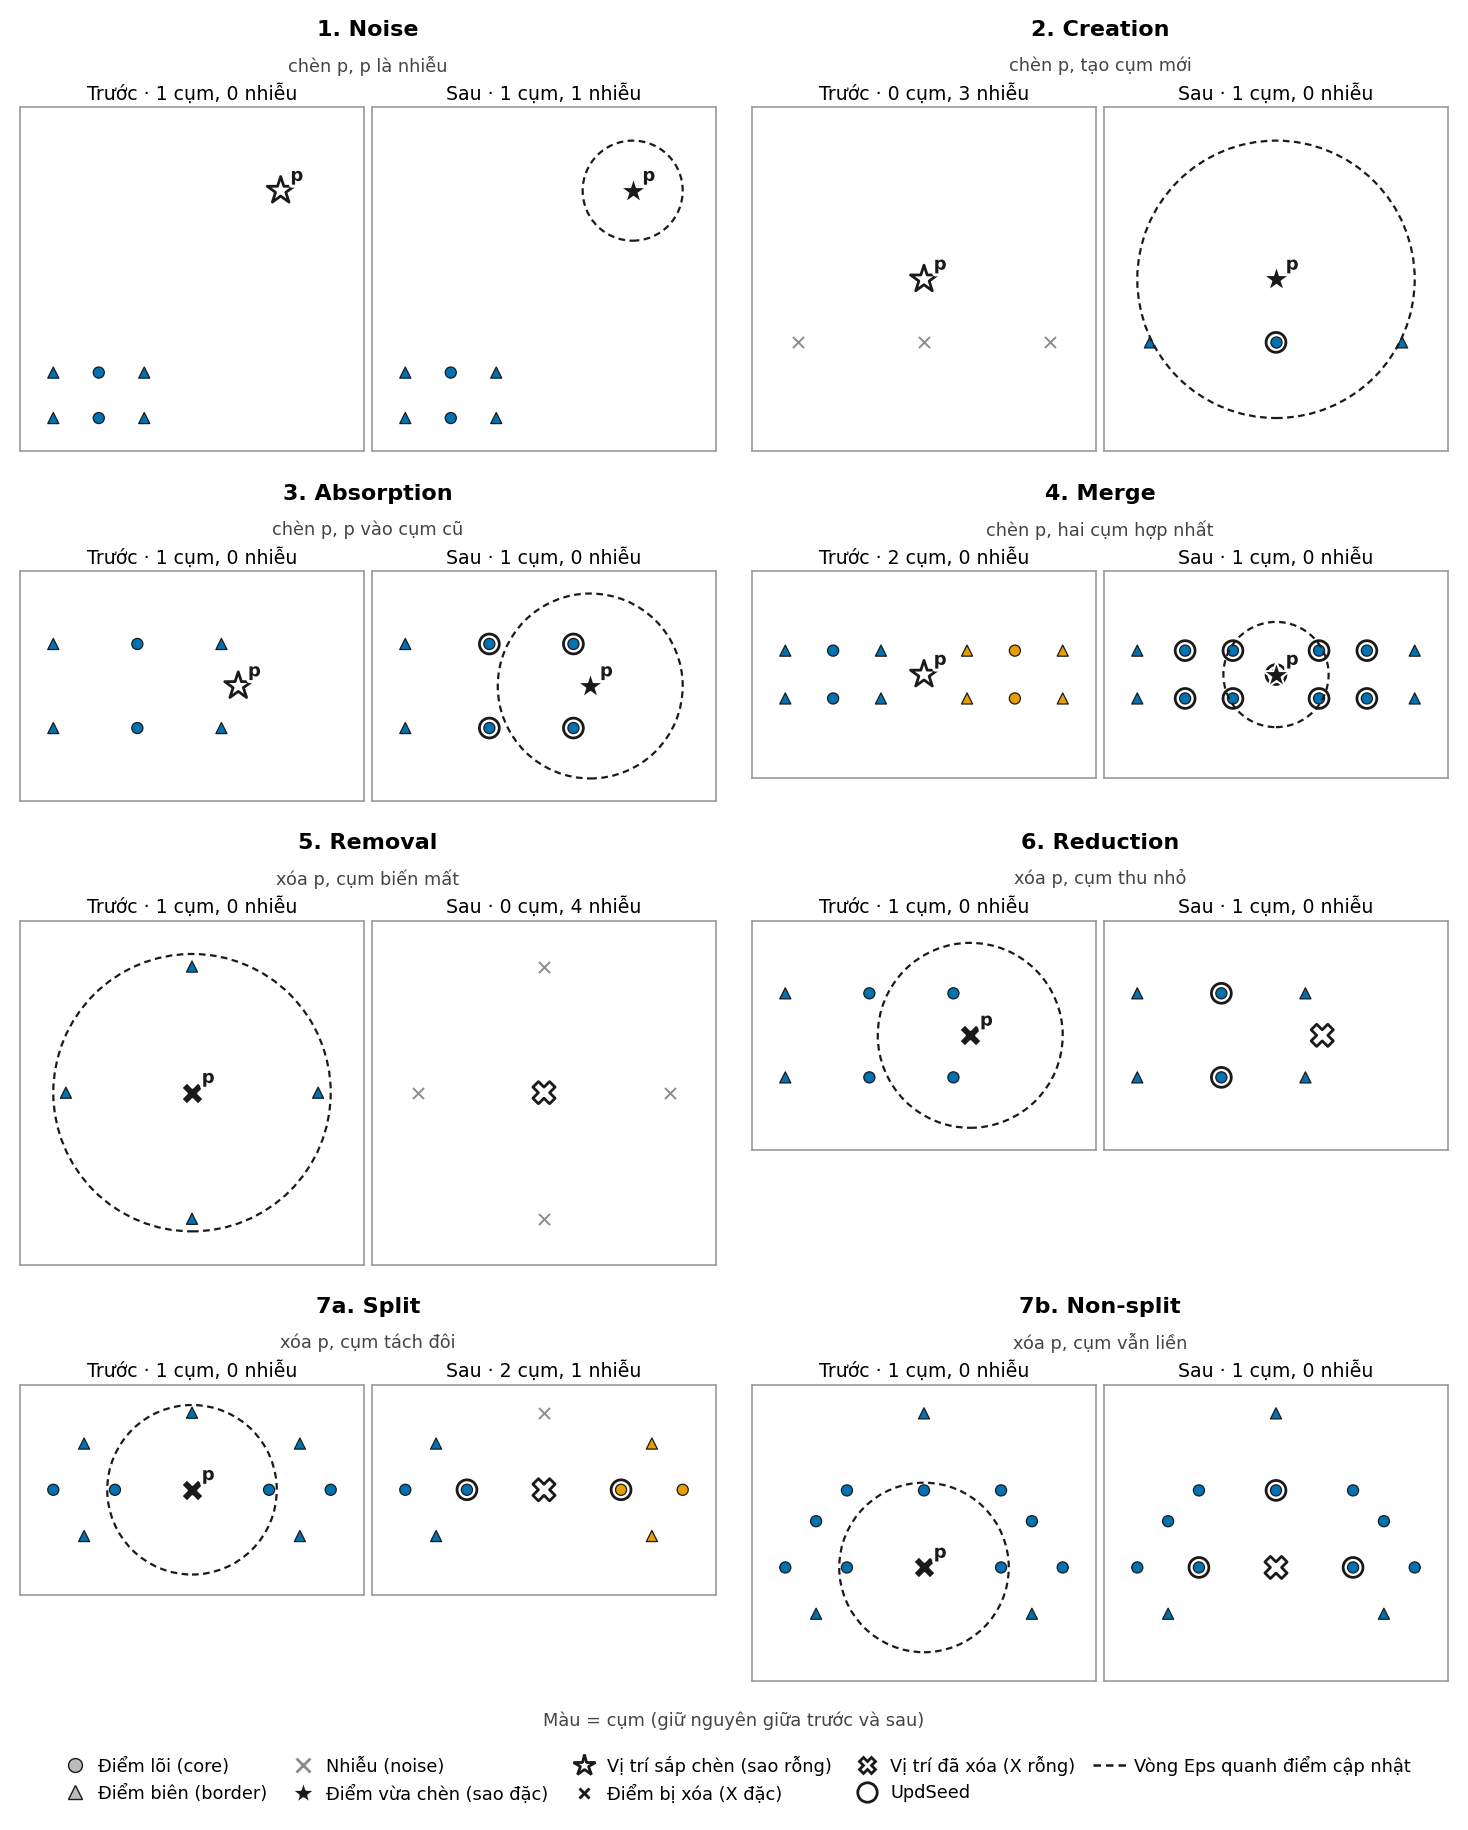
\includegraphics[
        width=\textwidth,
        trim=0bp 365bp 0bp 0bp,
        clip
    ]{Images/case_gallery_insert_delete.png}
    \caption{Minh họa các trường hợp cập nhật khi chèn đối tượng: Noise, Creation, Absorption và Merge}
    \label{fig:insert_cases}
\end{figure}

\textbf{Trường hợp 1 - Noise (Nhiễu)}

Trường hợp Noise xảy ra khi phép chèn không tạo ra lõi mới và đối tượng \(p\) không nằm trong lân cận của bất kỳ lõi nào đã tồn tại. Khi đó, \(p\) không đủ điều kiện để bắt đầu một cụm và cũng không thể gia nhập cụm cũ dưới dạng đối tượng biên.

Xét sáu đối tượng \(A=(0;0)\), \(B=(1;0)\), \(C=(2;0)\), \(D=(0;1)\), \(E=(1;1)\) và \(F=(2;1)\), với \(\varepsilon=1{,}1\) và \(\mathrm{MinPts}=4\).

Trước cập nhật, \(B\) và \(E\) là hai đối tượng lõi, các đối tượng còn lại là biên và toàn bộ sáu đối tượng thuộc cùng một cụm \(C_1\).

Chèn thêm đối tượng \(p=(5;5)\). Do khoảng cách từ \(p\) đến mọi đối tượng cũ đều lớn hơn \(\varepsilon\), ta có:

\begin{equation}
N_{\varepsilon}(p)=\{p\},
\qquad |N_{\varepsilon}(p)|=1<4.
\end{equation}

Không có đối tượng cũ nào tăng số lượng lân cận, nên \(\mathrm{NewCore}=\varnothing\). Đồng thời, \(p\) không nằm trong lân cận của lõi \(B\) hoặc \(E\).

Kết quả, \(p\) được xác định là nhiễu và cụm \(C_1\) không thay đổi.

Lưu ý: \(\mathrm{NewCore}=\varnothing\) chưa đủ để kết luận \(p\) là nhiễu. Nếu \(p\) nằm trong lân cận của một lõi cũ, nó vẫn có thể được bổ sung vào cụm dưới dạng đối tượng biên mà không làm xuất hiện lõi mới.

\textbf{Trường hợp 2 - Creation (Tạo cụm mới)}

Creation xảy ra khi phép chèn tạo ra một hoặc nhiều đối tượng lõi, nhưng những kết nối mới không dẫn đến bất kỳ cụm nào đã tồn tại trước cập nhật.

Xét ba đối tượng \(A=(0;0)\), \(B=(1;0)\) và \(C=(2;0)\), với \(\varepsilon=1{,}1\) và \(\mathrm{MinPts}=4\).

Trước khi chèn, số lượng đối tượng trong lân cận của \(A\), \(B\), \(C\) lần lượt là 2, 3 và 2. Vì không có đối tượng lõi, cả ba đều được xác định là nhiễu.

Chèn đối tượng \(p=(1;0{,}5)\). Khoảng cách từ \(p\) đến \(B\) bằng \(0{,}5\), trong khi khoảng cách đến \(A\) và \(C\) đều lớn hơn \(1{,}1\). Do đó:

\begin{equation}
    N_{\varepsilon}(p)=\{B,p\}.
\end{equation}

Đối tượng \(B\) có số lượng lân cận tăng từ 3 lên 4:

\begin{equation}
    |N_{\varepsilon}(B)|:3\longrightarrow4.
\end{equation}

Vì đạt ngưỡng \(\mathrm{MinPts}\), \(B\) chuyển từ nhiễu thành lõi. Khi đó:

\begin{equation}
    \mathrm{NewCore}=\{B\},
    \qquad
    \mathrm{UpdSeed}_{Ins}=\{B\}.
\end{equation}

Từ lõi \(B\), các đối tượng \(A\), \(C\) và \(p\) đều khả đạt trực tiếp theo mật độ. Vì trước đó chưa có cụm nào, thuật toán tạo cụm mới:

\begin{equation}
    C_1=\{A,B,C,p\}.
\end{equation}

Trong kết quả này, \(B\) là lõi, còn \(A\), \(C\) và \(p\) là biên. Phép chèn chỉ tạo ra một lõi mới nhưng đủ để hình thành cụm gồm bốn đối tượng.

\textbf{Trường hợp 3 - Absorption (Bổ sung vào cụm hiện có)}

Absorption xảy ra khi các kết nối được tạo thêm chỉ liên hệ với một cụm đã tồn tại. Cụm này được mở rộng mà không cần hợp nhất với cụm khác. Trường hợp này cũng có thể xảy ra khi phép chèn không tạo ra lõi mới, nhưng đối tượng được chèn nằm trong lân cận của một lõi đã tồn tại và được bổ sung vào cụm dưới dạng đối tượng biên.

Xét sáu đối tượng \(A=(0;0)\), \(B=(1;0)\), \(C=(0;1)\), \(D=(1;1)\), \(E=(2;0)\) và \(F=(2;1)\), với \(\varepsilon=1{,}1\) và \(\mathrm{MinPts}=4\).

Trước cập nhật, \(B\) và \(D\) là lõi, bốn đối tượng còn lại là biên. Toàn bộ dữ liệu thuộc cùng một cụm \(C_1\).

Chèn đối tượng \(p=(2{,}2;0{,}5)\). Đối tượng mới nằm trong lân cận của \(E\) và \(F\), làm số lượng lân cận của hai đối tượng này tăng từ 3 lên 4:

\begin{equation}
\begin{aligned}
    |N_{\varepsilon}(E)| &:3\longrightarrow4,\\
    |N_{\varepsilon}(F)| &:3\longrightarrow4.
\end{aligned}
\end{equation}

Do đó, \(E\) và \(F\) chuyển từ biên thành lõi. Trong khi đó, \(p\) có ba đối tượng trong lân cận là \(E\), \(F\) và chính nó, nên vẫn là biên.

Từ hai lõi mới, thuật toán xác định:

\begin{equation}
    \mathrm{NewCore}=\{E,F\},
\end{equation}

\begin{equation}
    \mathrm{UpdSeed}_{Ins}=\{B,D,E,F\}.
\end{equation}

Vì \(B\) và \(D\) đều thuộc \(C_1\) trước cập nhật, các kết nối mới không liên hệ với cụm thứ hai. Thuật toán giữ nhãn cụm hiện có và bổ sung \(p\):

\begin{equation}
    C_1'=\{A,B,C,D,E,F,p\}.
\end{equation}

Kết quả là số thành viên của cụm tăng từ sáu lên bảy. Đồng thời, hai đối tượng \(E\) và \(F\) thay đổi từ biên thành lõi, nhưng số lượng cụm vẫn là một.

\textbf{Trường hợp 4 - Merge (Hợp nhất cụm)}

Merge xảy ra khi các kết nối thông qua lõi mới liên hệ những đối tượng lõi thuộc ít nhất hai cụm khác nhau trước cập nhật. Khi đó, các cụm liên quan trở thành một cụm sau khi chèn.

Xét hai cụm ban đầu với \(\varepsilon=1{,}1\) và \(\mathrm{MinPts}=4\).

Cụm thứ nhất gồm sáu đối tượng:

\begin{equation}
\begin{aligned}
C_1=\{&
A_1=(-1;0),A_2=(0;0),A_3=(1;0),\\
&A_4=(-1;1),A_5=(0;1),A_6=(1;1)\}.
\end{aligned}
\end{equation}

Cụm thứ hai cũng gồm sáu đối tượng:

\begin{equation}
\begin{aligned}
C_2=\{&
B_1=(2{,}8;0),B_2=(3{,}8;0),B_3=(4{,}8;0),\\
&B_4=(2{,}8;1),B_5=(3{,}8;1),B_6=(4{,}8;1)\}.
\end{aligned}
\end{equation}

Trước cập nhật, \(A_2\), \(A_5\), \(B_2\) và \(B_5\) là các đối tượng lõi. Hai cụm chưa có kết nối theo mật độ.

Chèn đối tượng \(p=(1{,}9;0{,}5)\). Khoảng cách từ \(p\) đến các đối tượng \(A_3\), \(A_6\), \(B_1\), \(B_4\) đều bằng:

\begin{equation}
    \sqrt{0{,}9^2+0{,}5^2}
    =\sqrt{1{,}06}\approx1{,}03<1{,}1.
\end{equation}

Vì vậy:

\begin{equation}
N_{\varepsilon}(p)=\{p,A_3,A_6,B_1,B_4\}.
\end{equation}

Đối tượng \(p\) có năm phần tử trong lân cận nên trở thành lõi. Đồng thời, \(A_3\), \(A_6\), \(B_1\) và \(B_4\) đều tăng số lượng lân cận từ 3 lên 4, do đó cũng trở thành lõi.

Tập lõi mới gồm:

\begin{equation}
    \mathrm{NewCore}=\{p,A_3,A_6,B_1,B_4\}.
\end{equation}

Khi xác định các đối tượng lõi trong lân cận của \(\mathrm{NewCore}\), ta thu được:

\begin{equation}
\begin{aligned}
\mathrm{UpdSeed}_{Ins}=\{&
A_2,A_3,A_5,A_6,\\
&B_1,B_2,B_4,B_5,p\}.
\end{aligned}
\end{equation}

Tập này chứa các lõi thuộc cả \(C_1\) và \(C_2\). Đặc biệt, lõi \(p\) kết nối với những lõi mới ở hai phía, tạo ra đường kết nối mật độ giữa hai cụm.

Vì vậy, thuật toán hợp nhất \(C_1\), \(C_2\) và \(p\) thành một cụm gồm 13 đối tượng:

\begin{equation}
    C=C_1\cup C_2\cup\{p\}.
\end{equation}

Trong chương trình của nhóm, việc hợp nhất được thực hiện bằng cách giữ lại một nhãn cụm và cập nhật nhãn của các thành viên thuộc cụm còn lại. Thuật toán xác định những cụm cần hợp nhất dựa trên các kết nối mới giữa những đối tượng lõi, thay vì tính lại lân cận của toàn bộ 13 đối tượng. Tuy nhiên, chương trình vẫn cần duyệt các đối tượng đang lưu để cập nhật nhãn của những đối tượng thuộc cụm bị hợp nhất.

\subsection{Các trường hợp khi xóa điểm}

\textbf{Nguyên tắc cập nhật khi xóa}

Khi xóa một đối tượng \(p\), số lượng phần tử trong lân cận của những đối tượng còn lại chỉ có thể giảm hoặc giữ nguyên. Vì vậy, những đối tượng trước đó không phải lõi không thể trở thành lõi do phép xóa, ngược lại, một số đối tượng lõi có thể mất tính chất lõi.

Phép xóa không tạo thêm các kết nối theo mật độ. Tuy nhiên, việc mất một đối tượng lõi không nhất thiết khiến cụm bị tách, bởi các đối tượng còn lại vẫn có thể được liên kết thông qua những lõi khác.

Ba trường hợp chính khi xóa là Removal, Reduction và Potential Split. Riêng Potential Split cần phân biệt hai kết quả: Split và Non-split.

\begin{table}[H]
\centering
\caption{Các trường hợp cập nhật khi xóa đối tượng}
\label{tab:incremental_delete_cases}
\normalsize
\begin{tabularx}{\textwidth}{|P{2.8cm}|Y|Y|}
\hline
\textbf{Trường hợp} & \textbf{Đặc điểm} & \textbf{Kết quả} \\
\hline
Removal &
Tập UpdSeedDel rỗng, không có đối tượng lõi còn lại nằm trong lân cận của những đối tượng vừa mất tính chất lõi. &
Đối tượng bị xóa, một số đối tượng có thể trở thành nhiễu. Cụm có thể biến mất nếu không còn lõi.
\\
\hline
Reduction &
Các đối tượng thuộc UpdSeedDel đều khả đạt trực tiếp theo mật độ từ nhau sau phép xóa. &
Cụm vẫn được duy trì nhưng có thể giảm số thành viên hoặc thay đổi tính chất của một số đối tượng. \\
\hline
Potential Split &
Các đối tượng thuộc UpdSeedDel trước đó thuộc cùng một cụm nhưng không còn khả đạt trực tiếp theo mật độ từ nhau. &
Cần kiểm tra xem các đối tượng còn kết nối thông qua những lõi khác hay không, từ đó xác định Split hoặc Non-split. \\
\hline
\end{tabularx}
\end{table}

\textbf{Quy trình DELETE trong chương trình của nhóm}

Phương thức \texttt{delete()} cập nhật cụm quanh điểm bị xóa. Quy trình dưới đây theo các bước mà nhóm đã cài đặt:

\begin{enumerate}[label=\textbf{Bước \arabic*.}, leftmargin=*, itemsep=4pt]
    \item Tìm điểm \(p\) cần xóa và lưu thông tin lân cận, nhãn cụm, trạng thái lõi của các điểm liên quan.
    \item Xóa \(p\) và bỏ ID của nó khỏi danh sách lân cận của các điểm còn lại.
    \item Tìm các điểm lõi bị mất trạng thái lõi. Từ các điểm này, tạo tập \(\mathrm{UpdSeed}_{Del}\), gồm các điểm lõi còn lại cần kiểm tra.
    \item Xét từng cụm liên quan. Nếu không có seed thì đó là Removal. Nếu các seed kề trực tiếp với nhau thì đó là Reduction và cụm không cần tách.
    \item Nếu các seed không kề trực tiếp, dùng BFS để lần theo các điểm lõi. Nếu BFS nối được các seed thì cụm không tách (Non-split); nếu không, các phần lõi bị rời nhau được gán thành các cụm riêng (Split).
    \item Cập nhật nhãn của các điểm lõi thuộc cụm bị tách, rồi phân loại lại các điểm không lõi liên quan thành biên hoặc nhiễu.
\end{enumerate}

Các điểm biên không được dùng làm cầu nối giữa hai cụm. Vì vậy, chương trình xác định kết nối giữa các điểm lõi trước, rồi mới gán lại trạng thái và nhãn cho những điểm biên hoặc nhiễu bị ảnh hưởng.

Cách làm này cũng xử lý được trường hợp xóa một điểm biên hoặc xóa điểm mà không làm điểm lõi nào mất trạng thái lõi.

\begin{figure}[H]
    \centering
    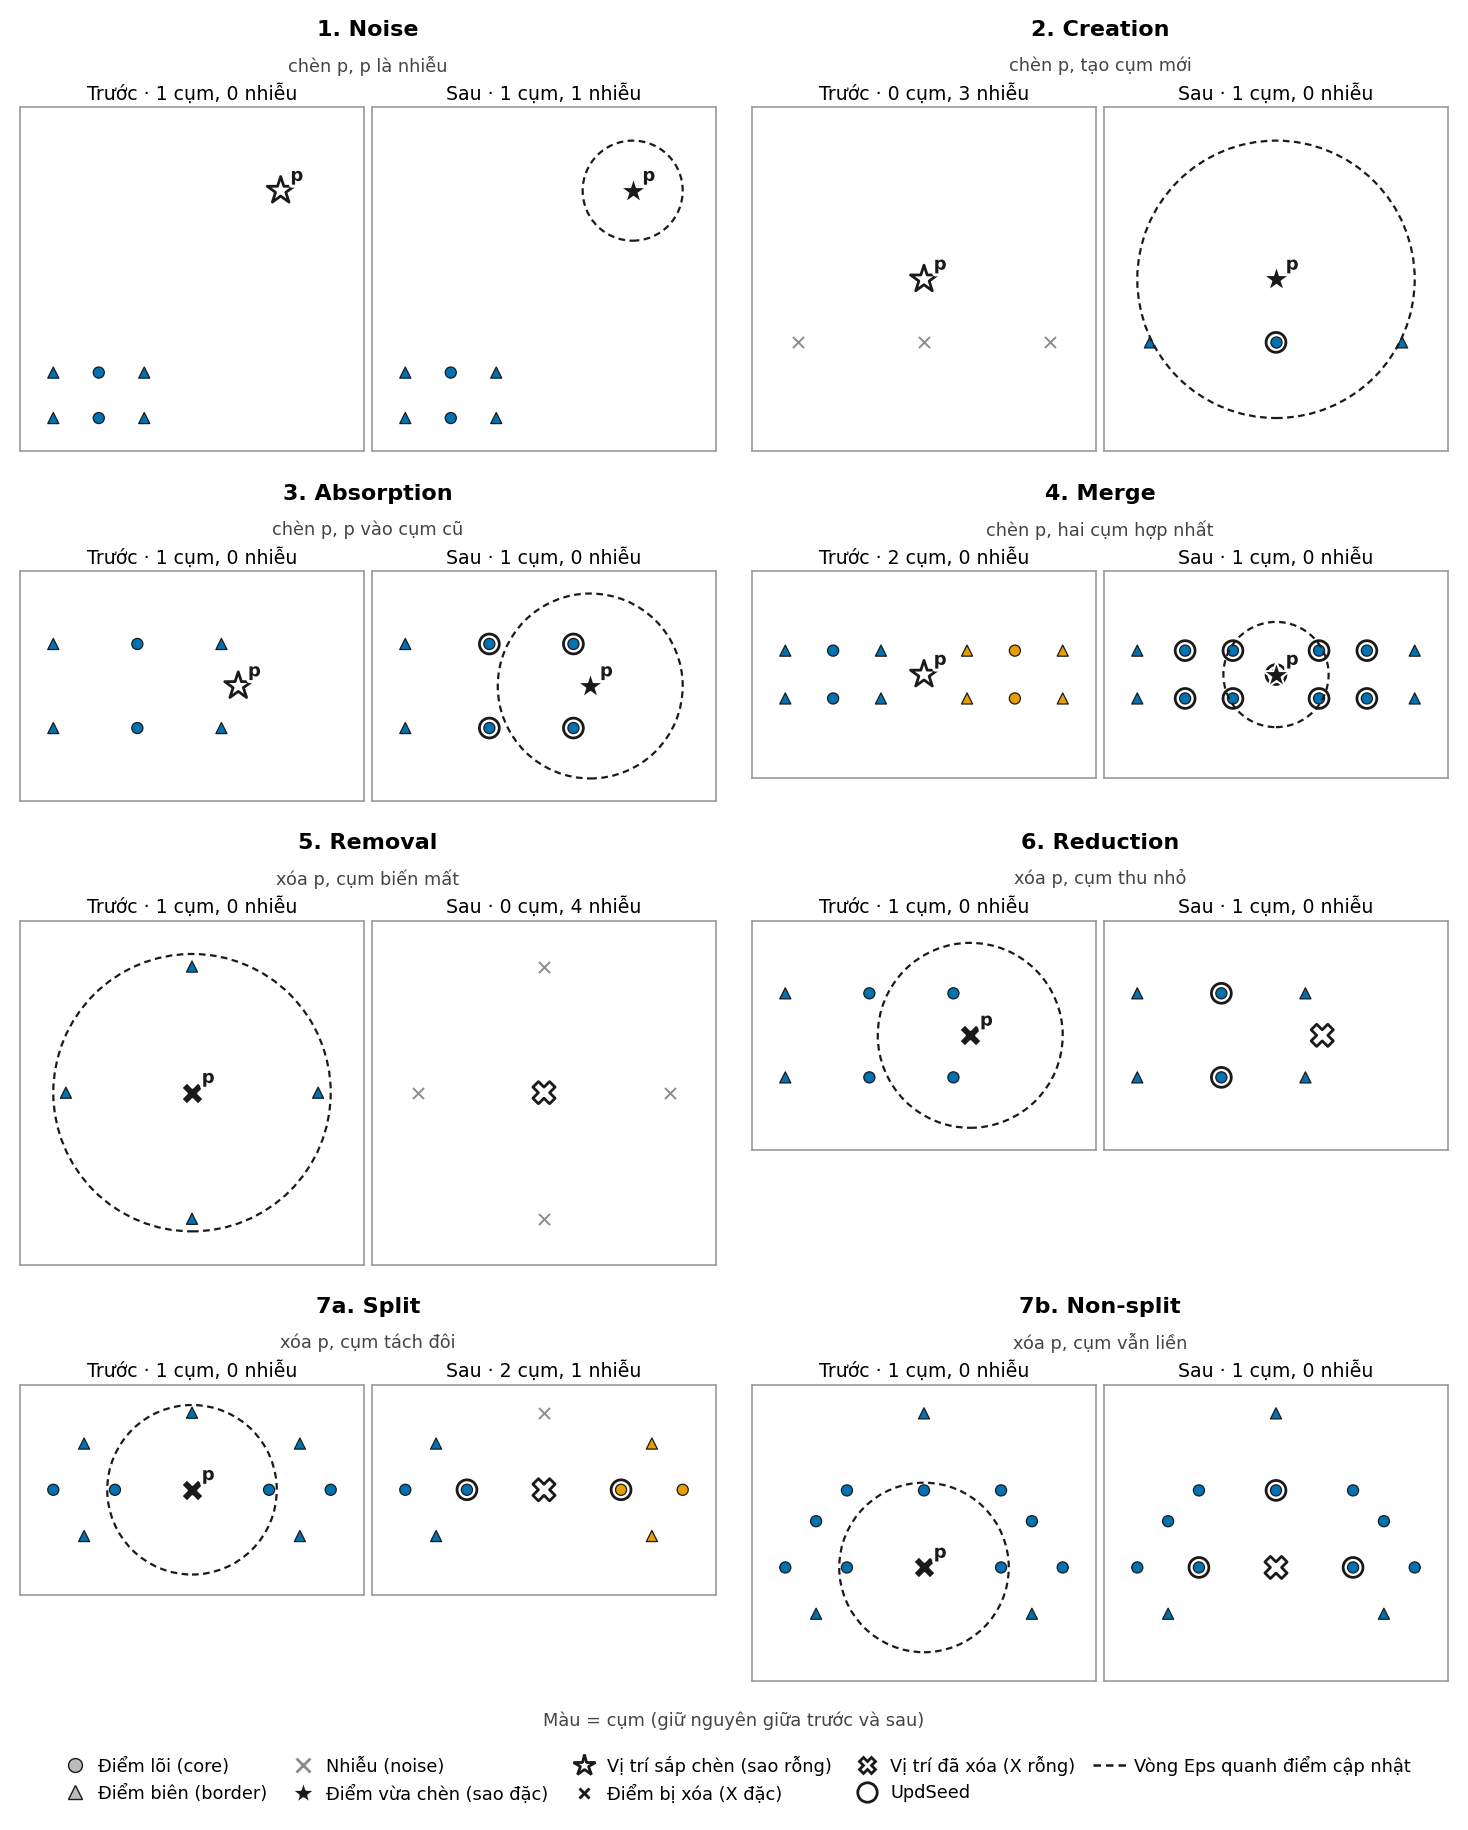
\includegraphics[
        width=\textwidth,
        trim=0bp 0bp 0bp 294bp,
        clip
    ]{Images/case_gallery_insert_delete.png}
    \caption{Minh họa các trường hợp cập nhật khi xóa đối tượng: Removal, Reduction, Split và Non-split}
    \label{fig:delete_cases}
\end{figure}

\textbf{Trường hợp 1 - Removal (Loại bỏ)}

Theo lý thuyết Incremental DBSCAN, Removal xảy ra khi tập UpdSeedDel rỗng, nghĩa là không còn đối tượng lõi nào trong lân cận của những đối tượng vừa mất tính chất lõi sau phép xóa. Khi đó, không cần tìm đường kết nối thay thế giữa các lõi. Nếu đối tượng bị xóa là lõi duy nhất duy trì một cụm, việc xóa có thể khiến cụm đó biến mất hoàn toàn.

Xét năm đối tượng:

\begin{equation}
\begin{aligned}
A&=(-1;0), & B&=(1;0),\\
C&=(0;-1), & D&=(0;1),\\
p&=(0;0).
\end{aligned}
\end{equation}

Với \(\varepsilon=1{,}1\) và \(\mathrm{MinPts}=4\), đối tượng \(p\) có lân cận:

\begin{equation}
N_{\varepsilon}(p)=\{A,B,C,D,p\}.
\end{equation}

Do có năm phần tử trong lân cận, \(p\) là lõi. Bốn đối tượng còn lại đều nằm trong lân cận của \(p\) nhưng không đủ điều kiện lõi, nên được xác định là biên. Tập dữ liệu ban đầu hình thành một cụm gồm năm đối tượng.

Sau khi xóa \(p\), các đối tượng \(A\), \(B\), \(C\), \(D\) không còn nằm trong lân cận của bất kỳ lõi nào. Mỗi đối tượng chỉ còn chính nó trong lân cận, vì khoảng cách giữa các đối tượng còn lại đều lớn hơn \(1{,}1\).

Khi đó, không còn đối tượng nào thỏa mãn điều kiện lõi, và:

\begin{equation}
    \mathrm{UpdSeed}_{Del}=\varnothing.
\end{equation}

Trong kết quả sau cập nhật, cụm ban đầu không còn tồn tại, bốn đối tượng còn lại đều trở thành nhiễu:

\begin{equation}
    {N}=\{A,B,C,D\}.
\end{equation}

Ví dụ cho thấy xóa một đối tượng không chỉ làm giảm số lượng thành viên của cụm. Nếu đối tượng đó là lõi duy nhất, phép xóa có thể loại bỏ toàn bộ cấu trúc cụm.

\textbf{Trường hợp 2 - Reduction (Thu hẹp cụm)}

Reduction xảy ra khi các đối tượng thuộc UpdSeedDel vẫn khả đạt trực tiếp theo mật độ từ nhau sau phép xóa. Điều này cho thấy những kết nối trực tiếp cần thiết giữa các đối tượng lõi liên quan vẫn được duy trì, nên không cần tìm kiếm đường kết nối thay thế. Một số đối tượng có thể mất tính chất lõi hoặc trở thành nhiễu, khiến cụm giảm số thành viên nhưng không bị tách thành các cụm riêng biệt.

Xét tập dữ liệu gồm:

\begin{equation}
\begin{aligned}
A&=(0;0), & B&=(1;0),\\
C&=(0;1), & D&=(1;1),\\
E&=(2;0), & F&=(2;1),\\
p&=(2{,}2;0{,}5).
\end{aligned}
\end{equation}

Với \(\varepsilon=1{,}1\) và \(\mathrm{MinPts}=4\), trước cập nhật, các đối tượng \(B\), \(D\), \(E\) và \(F\) là lõi. Toàn bộ bảy đối tượng thuộc cùng một cụm.

Khi xóa \(p\), số lượng lân cận của \(E\) và \(F\) giảm từ 4 xuống 3:

\begin{equation}
\begin{aligned}
    |N_{\varepsilon}(E)| &:4\longrightarrow3,\\
    |N_{\varepsilon}(F)| &:4\longrightarrow3.
\end{aligned}
\end{equation}

Vì vậy, \(E\) và \(F\) mất tính chất lõi, trong khi \(B\) và \(D\) vẫn là lõi. Hai đối tượng này cách nhau một đơn vị, nhỏ hơn \(\varepsilon\), nên vẫn khả đạt trực tiếp theo mật độ từ nhau.

Theo cách xác định trong paper:

\begin{equation}
    \mathrm{UpdSeed}_{Del}=\{B,D\}.
\end{equation}

Các đối tượng \(E\) và \(F\) vẫn nằm trong lân cận của lõi \(B\) hoặc \(D\), nên chuyển thành biên chứ không trở thành nhiễu.

Kết quả sau cập nhật là:

\begin{equation}
    C_1'=\{A,B,C,D,E,F\}.
\end{equation}

Cụm giảm từ bảy xuống sáu thành viên nhưng vẫn duy trì cấu trúc liên thông. Đây là trường hợp có sự thay đổi tính chất lõi nhưng không làm mất kết nối giữa những phần còn lại của cụm.

\textbf{Trường hợp 3 - Potential Split (Khả năng tách cụm)}

Potential Split xảy ra khi phép xóa làm mất những kết nối trực tiếp cần thiết giữa các đối tượng lõi. Tuy nhiên, việc mất kết nối trực tiếp chưa đủ để kết luận cụm bị tách, bởi vẫn có thể tồn tại đường kết nối thông qua những lõi khác.

Để xác định kết quả, cần kiểm tra các chuỗi kết nối giữa những đối tượng lõi còn lại. Có hai khả năng:

\begin{itemize}
    \item \textbf{Split:} Không còn đường kết nối lõi giữa một số phần của cụm, cụm ban đầu tách thành nhiều cụm.
    \item \textbf{Non-split:} Vẫn tồn tại đường kết nối lõi thay thế, cụm không bị tách.
\end{itemize}

\textbf{Trường hợp A - Split (Tách cụm)}

Xét mười đối tượng trong không gian hai chiều với \(\varepsilon=1{,}1\) và \(\mathrm{MinPts}=4\):

\begin{equation}
\begin{aligned}
A&=(1;0), & B&=(0{,}2;0),\\
C&=(0{,}6;0{,}6), & D&=(0{,}6;-0{,}6),\\
E&=(3;0), & F&=(3{,}8;0),\\
G&=(3{,}4;0{,}6), & H&=(3{,}4;-0{,}6),\\
I&=(2;1), & p&=(2;0).
\end{aligned}
\end{equation}

Trước khi xóa, \(A\), \(B\), \(E\), \(F\) và \(p\) là các đối tượng lõi. Trong đó, \(p\) nằm giữa hai vùng đối tượng và có lân cận:

\begin{equation}
    N_{\varepsilon}(p)=\{A,E,I,p\}.
\end{equation}

Do \(p\) là lõi, nó tạo ra kết nối mật độ giữa hai phía của cụm thông qua các đối tượng \(A\) và \(E\). Toàn bộ mười đối tượng ban đầu thuộc cùng một cụm.

Sau khi xóa \(p\), các đối tượng \(A\) và \(E\) vẫn là lõi với số lượng lân cận giảm từ 5 xuống 4. Tuy nhiên, khoảng cách giữa chúng là:

\begin{equation}
    d(A,E)=2>\varepsilon.
\end{equation}

Vì vậy, \(A\) và \(E\) không còn kết nối trực tiếp. Đồng thời, không tồn tại chuỗi đối tượng lõi thay thế nối hai phía sau khi loại bỏ \(p\).

Đối tượng \(I\) cũng không còn nằm trong lân cận của lõi nào và chuyển thành nhiễu.

Kết quả, cụm ban đầu tách thành hai cụm:

\begin{equation}
    C_1=\{A,B,C,D\},
\end{equation}

\begin{equation}
    C_2=\{E,F,G,H\},
\end{equation}

và tập nhiễu:

\begin{equation}
    N =\{I\}.
\end{equation}

Ví dụ cho thấy một đối tượng lõi có thể đóng vai trò nối hai phần của cùng một cụm. Khi đối tượng đó bị xóa và không còn chuỗi kết nối lõi thay thế, hai phần sẽ trở thành những cụm riêng biệt.

\textbf{Trường hợp B - Non-split (Không tách cụm)}

Sử dụng dữ liệu của trường hợp A và bổ sung ba đối tượng:

\begin{equation}
    J=(1;1),\qquad K=(3;1),\qquad L=(2;2).
\end{equation}

Các tham số \(\varepsilon=1{,}1\) và \(\mathrm{MinPts}=4\) được giữ nguyên. Trước cập nhật, toàn bộ 13 đối tượng thuộc cùng một cụm.

Sau khi xóa \(p\), đối tượng \(I\) vẫn là lõi vì lân cận còn bốn đối tượng là \(I\), \(J\), \(K\) và \(L\). Đồng thời, \(J\) và \(K\) cũng tiếp tục thỏa mãn điều kiện lõi.

Mặc dù kết nối trực tiếp thông qua \(p\) không còn, thuật toán xác định được chuỗi lõi thay thế:

\begin{equation}
    A\rightarrow J\rightarrow I\rightarrow K\rightarrow E.
\end{equation}

Khoảng cách giữa từng cặp đối tượng liên tiếp trong chuỗi đều bằng 1, không vượt quá \(\varepsilon\). Hơn nữa, tất cả đối tượng trong chuỗi đều là lõi sau cập nhật, nên các quan hệ khả đạt trực tiếp theo mật độ vẫn được duy trì dọc theo chuỗi.

Vì vậy, hai phía của cụm vẫn có quan hệ kết nối theo mật độ. Kết quả là 12 đối tượng còn lại tiếp tục thuộc cùng một cụm.

Hai ví dụ Split và Non-split cho thấy việc mất một đối tượng lõi không tự động dẫn đến tách cụm. Yếu tố quyết định là sau phép xóa có còn tồn tại đường kết nối thông qua những đối tượng lõi khác hay không.

Trong code, BFS bắt đầu từ các điểm trong \(\mathrm{UpdSeed}_{Del}\) và chỉ đi qua những điểm lõi còn kề nhau. Nếu đã tìm thấy đường nối giữa các seed thì chương trình dừng việc kiểm tra tách cụm. Nếu không tìm thấy đường nối, chương trình xác định các phần lõi bị tách và cập nhật nhãn của chúng. Như vậy, phần cài đặt có dùng \(\mathrm{UpdSeed}_{Del}\); BFS là bước kiểm tra kết nối sau khi tạo tập seed.

\subsection{Khác biệt giữa Incremental DBSCAN và chạy lại DBSCAN}

Incremental DBSCAN (cập nhật tăng dần)  và chạy lại DBSCAN đều nhằm xác định cấu trúc gom cụm phù hợp với tập dữ liệu sau thay đổi. Điểm khác nhau nằm ở lượng thông tin được sử dụng lại và phạm vi cần xử lý.

Đối với cách chạy lại DBSCAN, mỗi lần cập nhật được xem như một bài toán gom cụm mới. Thuật toán thực hiện lại việc xác định lân cận, tính chất lõi và mở rộng cụm trên tập dữ liệu hiện tại.

Trong khi đó, Incremental DBSCAN giữ lại thông tin về đối tượng, lân cận, loại đối tượng và nhãn cụm sau mỗi lần xử lý. Khi phát sinh phép chèn hoặc xóa, thuật toán cập nhật những thông tin có thay đổi và điều chỉnh các cụm liên quan.

\begin{table}[H]
\centering
\caption{So sánh cách cập nhật kết quả gom cụm}
\label{tab:incremental_vs_refit}
\normalsize
\begin{tabularx}{\textwidth}{|P{3.1cm}|Y|Y|}
\hline
\textbf{Tiêu chí} & \textbf{Chạy lại DBSCAN} & \textbf{Incremental DBSCAN của nhóm} \\
\hline
Thông tin ban đầu &
Gom cụm lại tập dữ liệu hiện tại. &
Sử dụng kết quả gom cụm và lân cận đã lưu. \\
\hline
Phép chèn &
Tính lại lân cận và mở rộng cụm trên toàn bộ dữ liệu. &
Cập nhật lân cận của điểm mới và những đối tượng liên quan, sau đó xử lý các kết nối mới. \\
\hline
Phép xóa &
Gom cụm lại toàn bộ dữ liệu còn lại. &
Xác định các cụm liên quan, kiểm tra lại các thành phần lõi và gán lại nhãn. \\
\hline
Bộ nhớ &
Phụ thuộc cách cài đặt và lưu trữ lân cận. &
Cần duy trì tập lân cận và trạng thái của từng đối tượng. \\
\hline
Chi phí cập nhật &
Phụ thuộc quy mô toàn bộ tập dữ liệu sau thay đổi. &
Phụ thuộc phạm vi các cụm liên quan, chi phí duy trì trạng thái và những thao tác duyệt dữ liệu cần thiết để cập nhật nhãn cụm.\\
\hline
\end{tabularx}
\end{table}

Nhờ lưu lại thông tin lân cận và trạng thái phân cụm, Incremental DBSCAN có thể hạn chế việc tính toán lại toàn bộ dữ liệu sau mỗi phép chèn hoặc xóa. Tuy nhiên, trong một số trường hợp như hợp nhất hoặc tách cụm, chương trình vẫn phải duyệt lại nhiều đối tượng để cập nhật nhãn và kiểm tra các kết nối còn lại.

Việc duy trì trạng thái cũng làm tăng nhu cầu lưu trữ so với những cách cài đặt không giữ lại toàn bộ thông tin lân cận. Vì vậy, Incremental DBSCAN không nhất thiết xử lý nhanh hơn DBSCAN chạy lại trong mọi tình huống. Lợi ích của phương pháp phụ thuộc vào phạm vi dữ liệu bị ảnh hưởng và lượng thông tin có thể tái sử dụng sau mỗi cập nhật.

\section{Các chỉ số đánh giá}

Nhóm xem kết quả theo ba khía cạnh: cập nhật có đúng không, các cụm có tách biệt không, và mất bao lâu để chạy. Silhouette là chỉ số chính để nhận xét chất lượng cụm; ARI chỉ giúp đối chiếu tính đúng đắn với DBSCAN chạy lại.

Nhóm cũng ghi nhận thời gian chạy, số cụm và tỷ lệ nhiễu để mô tả kết quả. Bộ nhớ được nhận xét qua lượng trạng thái thuật toán phải lưu; nhóm không đo bộ nhớ thành một thí nghiệm riêng.

\subsection{Adjusted Rand Index (ARI)}

Adjusted Rand Index (ARI) là chỉ số đo mức độ tương đồng giữa hai kết quả phân cụm trên cùng một tập dữ liệu. Chỉ số này dựa trên việc xem xét các cặp đối tượng có được xếp vào cùng nhóm hoặc khác nhóm trong cả hai kết quả hay không, đồng thời hiệu chỉnh mức độ tương đồng có thể xuất hiện do ngẫu nhiên.

Giá trị ARI được diễn giải như sau:

\begin{itemize}
    \item ARI = 1: Hai kết quả có cùng cách phân nhóm, không phụ thuộc vào giá trị số của nhãn cụm.
    \item ARI \(\approx 0\): Mức độ tương đồng xấp xỉ giá trị kỳ vọng khi phân nhóm ngẫu nhiên.
    \item ARI < 0: Mức độ tương đồng thấp hơn giá trị kỳ vọng nói trên.
\end{itemize}

Trong đồ án, ARI chỉ dùng để kiểm tra kết quả Incremental DBSCAN có gần với DBSCAN chạy lại trên cùng dữ liệu, khoảng cách và tham số hay không. Các điểm nhiễu vẫn được giữ lại; nhãn \(-1\) được xem là một nhãn riêng trong phép đối chiếu. ARI không phải chỉ số chính để đánh giá chất lượng cụm.

Tuy nhiên, ARI không phân biệt trực tiếp đối tượng lõi và đối tượng biên. Ngoài ra, một đối tượng biên có thể được gán hợp lệ vào nhiều cụm khác nhau. Vì vậy, nhóm còn kiểm tra riêng tính chất lõi, trạng thái nhiễu và các trường hợp gán cụm của đối tượng biên, thay vì chỉ dựa vào ARI.

\subsection{Silhouette}

Silhouette cho biết một điểm gần với cụm của nó đến mức nào và cách các cụm khác bao xa. Chỉ số này không cần nhãn đáp án có sẵn.

Với mỗi điểm \(i\), gọi \(a(i)\) là khoảng cách trung bình đến các điểm khác trong cùng cụm, còn \(b(i)\) là khoảng cách trung bình nhỏ nhất đến một cụm khác. Silhouette của điểm đó được tính như sau:

\begin{equation}
    s(i)=\frac{b(i)-a(i)}{\max\{a(i),b(i)\}}.
\end{equation}

Giá trị gần 1 thường có nghĩa điểm nằm gần cụm của mình và xa cụm khác; gần 0 là điểm nằm giữa các cụm; giá trị âm cho thấy điểm có thể gần cụm khác hơn cụm đang được gán.

Giá trị Silhouette nằm trong khoảng từ -1 đến 1, cụ thể như sau:

\begin{itemize}
    \item Gần 1: Đối tượng nằm gần các thành viên cùng cụm và tách biệt tương đối rõ với những cụm khác.
    \item Gần 0: Đối tượng có mức độ gần tương tự với cụm hiện tại và một cụm khác, cho thấy sự phân biệt giữa các cụm chưa rõ ràng.
    \item Gần -1: Đối tượng có xu hướng nằm gần một cụm khác hơn so với cụm hiện tại, có thể cho thấy việc gán cụm chưa phù hợp.
\end{itemize}

Silhouette của toàn bộ kết quả gom cụm được xác định bằng cách lấy trung bình giá trị Silhouette của các đối tượng được đưa vào đánh giá. Giá trị trung bình càng cao thường cho thấy các cụm càng tập trung và tách biệt rõ theo khoảng cách sử dụng.

\textbf{Cách nhóm tính Silhouette}

Nhóm tự cài phép tính Silhouette theo công thức trên. Các điểm nhiễu có nhãn \(-1\) được bỏ khỏi phép tính, còn các điểm thuộc cụm được giữ lại.

Chỉ tính điểm tổng hợp khi sau khi bỏ nhiễu còn ít nhất hai cụm. Nếu điều kiện này không đạt, kết quả được ghi là chưa xác định. Nếu một cụm chỉ có một điểm, Silhouette của điểm đó được quy ước bằng 0. Vì bỏ nhiễu có thể làm điểm trung bình tăng, nhóm đọc Silhouette cùng số cụm và tỷ lệ nhiễu.

\textbf{Giới hạn khi đánh giá DBSCAN bằng Silhouette}

Silhouette phản ánh sự gần nhau và tách biệt giữa các cụm dựa trên khoảng cách trung bình, nên thường thuận lợi cho những cụm có các đối tượng phân bố tập trung và cách xa nhau. Trong khi đó, DBSCAN có thể xác định những cụm có hình dạng không lồi. Với những dạng phân bố này, các đối tượng trong cùng cụm có thể cách nhau xa về mặt hình học nhưng vẫn được kết nối theo mật độ.

Vì vậy, Silhouette thấp không nhất thiết cho thấy DBSCAN gom cụm sai. Một kết quả phản ánh đúng các vùng kết nối theo mật độ vẫn có thể nhận Silhouette thấp hơn cách phân chia thành các cụm nhỏ, gọn hơn \parencite{sklearnClusteringGuide}.

Ngoài ra, khi loại nhiều đối tượng nhiễu khỏi phép tính, Silhouette trung bình có thể tăng do chỉ còn các đối tượng được gom vào những cụm rõ ràng hơn. Do đó, nhóm cần báo cáo Silhouette cùng số lượng hoặc tỷ lệ nhiễu để tránh đánh giá kết quả chỉ dựa trên những đối tượng được giữ lại.

\subsection{Thời gian chạy và bộ nhớ}

Thời gian thực hiện là một tiêu chí để đánh giá hiệu quả xử lý của Incremental DBSCAN. Khi so sánh với DBSCAN chạy lại, cần phân biệt thời gian gom cụm ban đầu và thời gian xử lý từng phép cập nhật. Chi phí cập nhật có thể thay đổi tùy theo loại thao tác và phạm vi cụm bị ảnh hưởng, do đó Incremental DBSCAN không nhất thiết nhanh hơn trong mọi trường hợp.

Bên cạnh thời gian xử lý, việc duy trì thông tin lân cận và trạng thái phân cụm cũng làm tăng nhu cầu bộ nhớ. Đây là sự đánh đổi giữa việc lưu trữ thông tin để tái sử dụng và việc phải tính toán lại từ đầu. Trong phạm vi đồ án, nhóm tập trung đo thời gian thực nghiệm, còn chi phí bộ nhớ được xem xét thông qua đặc điểm lưu trữ của thuật toán.

\subsection{Số cụm và số điểm nhiễu}

Số lượng cụm và số đối tượng nhiễu là những chỉ số mô tả trực tiếp kết quả gom cụm. Đối với Incremental DBSCAN, hai đại lượng này còn giúp theo dõi sự thay đổi cấu trúc dữ liệu sau mỗi phép chèn hoặc xóa.

Số cụm được xác định bằng cách đếm số nhãn cụm phân biệt trong kết quả, không tính nhãn -1 biểu thị nhiễu. Chẳng hạn, nếu tập dữ liệu có các nhãn {2, 2, 5, 5, -1}, kết quả gồm hai cụm và một đối tượng nhiễu. Số cụm được xác định dựa trên số nhãn phân biệt, không phụ thuộc vào giá trị cụ thể của các nhãn.

Số đối tượng nhiễu là số đối tượng mang nhãn -1 trong tập dữ liệu hiện tại. Tỷ lệ nhiễu cho biết tỷ lệ đối tượng không được gán vào cụm nào.

Đối với các phép cập nhật, nhóm theo dõi số cụm và số đối tượng nhiễu trước và sau thao tác để xác định những thay đổi trong kết quả gom cụm. Tuy nhiên, sự tăng hoặc giảm số cụm chưa đủ để xác định cụ thể trường hợp cập nhật đã xảy ra. Chẳng hạn, số cụm giảm có thể do hợp nhất hai cụm sau phép chèn hoặc do một cụm biến mất hoàn toàn sau phép xóa.

Tương tự, số đối tượng nhiễu tăng hoặc giảm có thể phản ánh sự thay đổi giữa trạng thái nhiễu và biên khi mật độ lân cận thay đổi. Vì vậy, nhóm kết hợp các đại lượng này với thông tin về loại đối tượng và quan hệ thành viên cụm để phân tích từng kịch bản.

Đối với các bộ dữ liệu mô phỏng có đối tượng nhiễu được xác định trước, số lượng và tỷ lệ nhiễu còn hỗ trợ đánh giá khả năng nhận diện các đối tượng nằm ngoài cấu trúc cụm.

\section{Các thuật toán dùng để so sánh}

Nhóm chọn DBSCAN, OPTICS và HDBSCAN để so sánh vì cả ba đều dựa trên mật độ nhưng tìm cụm theo những cách khác nhau. DBSCAN là đối chứng gần nhất với thuật toán nhóm tự cài. OPTICS và HDBSCAN giúp xem kết quả của hai cách phân cụm mật độ khác. Nhóm không đưa K-Means vào bảng so sánh chính vì K-Means thuộc cách phân cụm khác và không xử lý nhiễu như DBSCAN.

DBSCAN sử dụng hai tham số \(\varepsilon\) và \(\mathrm{MinPts}\) để xác định các đối tượng lõi và mở rộng cụm. OPTICS xây dựng thứ tự xử lý cùng khoảng cách khả đạt (Reachability Distance), qua đó hỗ trợ xem xét cấu trúc cụm ở nhiều ngưỡng mật độ. Trong khi đó, HDBSCAN xây dựng cấu trúc phân cấp dựa trên mật độ và lựa chọn những cụm có mức ổn định phù hợp, giúp nhận diện các cụm có mật độ khác nhau trong nhiều trường hợp \parencite{sklearnClusteringGuide}.

Trong benchmark, DBSCAN, HDBSCAN và OPTICS được lấy từ scikit-learn; sau mỗi cập nhật, các bản này được chạy lại trên toàn bộ dữ liệu hiện có. scikit-learn không cung cấp thao tác INSERT/DELETE tăng dần cho DBSCAN. Vì vậy, phép đo thời gian đối chiếu cập nhật cục bộ của chương trình nhóm với cách chạy lại toàn bộ, chứ không phải so sánh bốn thuật toán incremental.

Incremental DBSCAN vẫn dùng nguyên tắc mật độ của DBSCAN, nhưng tận dụng thông tin lân cận và cụm đã lưu để cập nhật sau INSERT hoặc DELETE.

Bảng~\ref{tab:clustering_algorithm_comparison} tổng hợp những đặc điểm chính của các thuật toán.

\begin{table}[H]
\centering
\caption{So sánh đặc điểm của các thuật toán gom cụm}
\label{tab:clustering_algorithm_comparison}
\normalsize
\begin{tabularx}{\textwidth}{|P{2.6cm}|Y|Y|}
\hline
\textbf{Thuật toán} &
\textbf{Nguyên tắc gom cụm} &
\textbf{Đặc điểm chính} \\
\hline
DBSCAN &
Kết nối các đối tượng theo mật độ với \(\varepsilon\) và \(\mathrm{MinPts}\). &
Nhận diện cụm không lồi và nhiễu; khó xử lý các cụm có mật độ chênh lệch lớn. \\
\hline

Incremental DBSCAN &
Tận dụng kết quả DBSCAN đã có để cập nhật cấu trúc cụm sau INSERT hoặc DELETE. &
Hỗ trợ chèn, xóa và sử dụng lại trạng thái, vẫn có thể cần duyệt nhiều đối tượng khi cập nhật nhãn cụm. \\
\hline

OPTICS &
Sắp xếp các đối tượng theo cấu trúc mật độ và khoảng cách khả đạt. &
Hỗ trợ phân tích cấu trúc cụm ở nhiều ngưỡng mật độ. \\
\hline

HDBSCAN &
Xây dựng và lựa chọn cụm từ cấu trúc phân cấp theo mật độ. &
Có thể nhận diện các cụm có mật độ khác nhau và xác định nhiễu. \\
\hline
\end{tabularx}
\end{table}
